%% Author_tex.tex
%% V1.0
%% 2012/13/12
%% developed by Techset
%%
%% This file describes the coding for rsproca.cls

\documentclass[openacc]{rsproca_new}%%%%where rsproca is the template name
\usepackage{anyfontsize}
\usepackage{amsmath}
\usepackage{amssymb}                % AMS symbols package
\usepackage{microtype}              % Micro-typography for sorting out spacing
\usepackage[utf8]{inputenc}
\usepackage[numbers]{natbib}
\usepackage[titletoc]{appendix}
\RequirePackage{xcolor}
\usepackage{pgfplots}
\pgfplotsset{compat=newest}
\usepackage{import}
\usepgfplotslibrary{groupplots}
\usepackage{graphicx}
\usepackage{subcaption}
\allowdisplaybreaks
\usetikzlibrary{shapes,arrows,chains}
%\PreviewEnvironment{tikzpicture}

\pgfplotsset{compat=newest}
\usepgfplotslibrary{units}
\usetikzlibrary{arrows,shapes,positioning}
%%%% *** Do not adjust lengths that control margins, column widths, etc. ***
% Useful shortcuts
\def\real{\mathbb{R}}
\def\complex{\mathbb{C}}
\def\integer{\mathbb{Z}}
\def\natural{\mathbb{N}}
\makeatletter
\def\diff{\@ifnextchar[{\@diffwith}{\@diffwithout}}
\def\@diffwith[#1]#2#3{\frac{\md^{#1} #2}{\md #3^{#1}}}
\def\@diffwithout#1#2{\frac{\md #1}{\md #2}}
\def\pdiff{\@ifnextchar[{\@pdiffwith}{\@pdiffwithout}}
\def\@pdiffwith[#1]#2#3{\frac{\partial^{#1} #2}{\partial #3^{#1}}}
\def\@pdiffwithout#1#2{\frac{\partial #1}{\partial #2}}
\makeatother
\def\pdifff#1#2#3{\frac{\partial^2 #1}{\partial #2\partial #3}}
\def\etal{\textit{et al}}
\def\rb#1{\left(#1\right)}
\def\bb#1{\left\{#1\right\}}
\def\sb#1{\left[#1\right]}
\def\tb#1{\left<#1\right>}
\def\abs#1{\left|#1\right|}
\def\norm#1{\left\|#1\right\|}
\def\half{{\textstyle\frac12}}

% Use the nice looking epsilon
\def\epsilon{\varepsilon}

% Boldface for vectors
\def\vec#1{\ensuremath{\mathbf{#1}}}

%%%%%%%%%%% New Commands %%%%%%%%%%%

% Referencing
\newcommand{\eref}[1]{(\ref{#1})}
\newcommand{\Eref}[1]{(\ref{#1})}
\newcommand{\ssref}[1]{subsection~\ref{#1}}
\newcommand{\Ssref}[1]{Subsection~\ref{#1}}
\newcommand{\sref}[1]{section~\ref{#1}}
\newcommand{\Sref}[1]{Section~\ref{#1}}
\newcommand{\cref}[1]{chapter~\ref{#1}}
\newcommand{\Cref}[1]{Chapter~\ref{#1}}
\newcommand{\fref}[1]{figure~\ref{#1}}
\newcommand{\Fref}[1]{Figure~\ref{#1}}
\newcommand{\frefs}[1]{figures~\ref{#1}}
\newcommand{\Frefs}[1]{Figures~\ref{#1}}
\newcommand{\tref}[1]{table~\ref{#1}}
\newcommand{\Tref}[1]{Table~\ref{#1}}
\newcommand{\asref}[1]{Assumption~\ref{#1}}
\newcommand{\Lref}[1]{Lemma~\ref{#1}}
\newcommand{\rref}[1]{Remark~\ref{#1}}


%%%%%%%%%%% Defining Enunciations  %%%%%%%%%%%
\newtheorem{theorem}{\bf Theorem}[section]
\newtheorem{condition}{\bf Condition}[section]
\newtheorem{corollary}{\bf Corollary}[section]
\newtheorem{lemma}{\bf Lemma}[section]
\newtheorem{definition}{\bf Definition}[section]
\newtheorem{assumption}{\bf Assumption}[section]
\newtheorem{remark}{\bf Remark}[section]

%%%%%%%%%%%%%%%%%%%%%%%%%%%%%%%%%%%%%%%%%%%%%%%

%%%% Adding dot after Reference number %%%%
\makeatletter
\renewcommand\@biblabel[1]{#1.}
\makeatother
\graphicspath{ {./Images/} }



\begin{document}
%%%% Article title to be placed here



\title{Exploring features of dynamical system near Hopf bifurcation using control based continuation}

\author{%%%% Author details
K.H. Lee$^{1}$, D.A.W. Barton$^{1}$ and L. Renson$^{1}$}

%%%%%%%%% Insert author address here
\address{$^{1}$Department of Engineering Mathematics, University of Bristol\\}

%%%% Subject entries to be placed here %%%%
\subject{mechanical engineering, differential equations}

%%%% Keyword entries to be placed here %%%%
\keywords{Hopf bifurcation, feedback control, limit cycle, stabilization}

%%%% Insert corresponding author and its email address}
\corres{K.H. Lee\\
\email{jz18526@bristol.ac.uk}}

%%%% Abstract text to be placed here %%%%%%%%%%%%
\begin{abstract}
 Limit cycle oscillation (LCO) of the self-excited system often cause a significant problem in various engineering applications. Therefore, exploring dynamic features such as the family of periodic orbits by experimental methods can help researchers to verify or identify the dynamic model of the self-excited system. In this paper, the control based continuation (CBC) scheme for Hopf bifurcation, which is the most common example of a self-excited system, is developed. CBC is an experimental scheme to explore the features of a dynamical system as the system parameter is varied. Feed-back control plays a critical role in stabilizing the unstable periodic response of the dynamical system in the CBC scheme. We show theoretically and experimentally how feed-back control can stabilize unstable LCO of the dynamical system near Hopf bifurcation. The scheme is applied to a flutter rig, and the CBC results are used to verify the linearized dynamical model and to identify the grey-box model.
\end{abstract}
%%%%%%%%%%%%%%%%%%%%%%%%%%%

\maketitle

\section{Introduction}\label{int}

Hopf bifurcation is problematic in many engineering applications such as flutter of aircraft wings and shimmying in wheels, where small perturbation to an equlibrium state can produce large displacement LCO response. Prototype of flying wing Hellios \cite{noll2004investigation} and Facebook's Aquila UAV crash would be the devastating example of Hopf bifurcation. Hopf bifurcation would be the typical example of a self-excited system produced by loss of stability of equilibrium with parameter variation and birth of a family of LCO near the bifurcation point. LCO is either stable (supercritical Hopf bifurcation) or unstable (subcritical Hopf bifurcation) close to Hopf bifurcation. The scenario of Hopf bifurcation is theoretically well established and can be found in the standard dynamical system textbooks \cite{kuznetsov2013elements}, and analysis tool for Hopf bifurcation is well developed for mathematical models such as normal form \cite{yu2002simplest,ashwin1995numerical} and numerical continuation methods \cite{doedel2000auto2000,dankowicz2013recipes}.

A dynamical system with Hopf bifurcation is often investigated experimentally to test such as flutter speeds of wing structure of the airplane. However, It is essential to stabilize the unstable LCO, which has valuable information about the system, to investigate the dynamical system. Feedback control can be used as a tool to stabilize the unstable LCO of the dynamical system when it is noninvasive. Time-delayed feedback control \cite{pyragas2006delayed,sieber2016generic} is popular feedback control scheme that feeds a signal $x(t)-x(t-T)$ back where $x(t)$ is output of the experiment and $T$ is period of the periodic orbit subject to be stabilized. Control-based continuation (CBC) resembles the approach of time-delayed feedback control by replacing delay signal $x(t-T)$ to time-periodic signal $x^*(t)$ which also reduces difficulties dealing with delayed signals such as memory problems and measurement noise. CBC scheme is generally solving fixed point problem experimentally, which is based on finding a noninvasive control target that stabilizes the unstable periodic orbit of the uncontrolled system. CBC was initially proposed by Sieber and Krauskopf \cite{sieber2008control} and applied to a wide range of experiments, especially mechanical system experiments. It was applied to parametrically excited pendulum \cite{sieber2011control}, impact oscillators \cite{bureau2013experimental,bureau2014experimental}, nonlinear energy harvester \cite{barton2013systematic,barton2011numerical}
, and cantilever beam with a nonlinear mechanism at its free tip \cite{renson2019application}. Also, CBC has been proved to produce critical information about nonlinear dynamical systems such as nonlinear normal modes \cite{renson2016robust,renson2016experimental} and floquet multipliers \cite{barton2017control} and harmonically coupled modes \cite{renson2019application}.

The experiment of the dynamical system is critical to researchers since it can be used to verify the mathematical model or even building one. Building a mathematical model from the experiment, well known as system identification, is a good way to find a way to improve the design of a system with bifurcation. Many nonparametric and parametric system identification methods have been developed and applied to various nonlinear dynamical systems. However, nonparametric nonlinear system identification methods like nonlinear auto-regressive moving average models with exogenous inputs (NARMAX) are not generally well applicable to problems with bifurcation behavior \cite{thothadri2005nonlinear}. Moreover, nonparametric models are not related to a physical model and computationally expensive to identify compared to parametric models. Hence, parametric methods are typically adopted in system identification of dynamical system with Hopf bifurcation. In \cite{fichera2014experimental}, modal analysis is used to identify the parameters of the equation of motion. Also, experimentally measured LCO response can be used to identify the parameters of the nonlinear equations \cite{abdelkefi2013analytical}.

The main contribution of this paper is the development of CBC scheme for Hopf bifurcation and providing the theoretical basis of the scheme. In other studies, experimental schemes were only discussed theoretically and numerically \cite{brown2011time,postlethwaite2013feedback}, particularly for the time-delayed feedback control scheme, for the system with Hopf bifurcation since it has limitation in the experimental application when the period of unstable LCO is unknown. However, we provide a novel CBC scheme which is applicable in real experiments to overcome difficulties of time-delayed feedback control in the experiment.

Another contribution of this paper is developing a framework of system identification using the result of CBC. Few studies \cite{abdelkefi2013analytical,thothadri2005nonlinear} can be foundin the context of system identification of system with Hopf bifurcation. However, this is the first research to build a mathematical model from an experiment of a subcritical Hopf bifurcation.

Rest of the paper is formulated as follows. In the second section, the general idea of CBC scheme is presented. In the third section, theory to simplify the dynamics of Hopf bifurcation is introduced, and we show that CBC applied to Hopf bifurcation is equivalent to forced Hopf bifurcation with single harmonic forcing if weakly nonlinear transformation is assumed. CBC scheme to lock the phase between the control target and the output response is presented and effective experimental scheme to find the stabilizability of the controller and to find noninvasive periodic solution is developed from the forced Hopf bifurcation. In the fourth section, the proposed CBC scheme is applied experimentally to a flutter rig that has subcritical Hopf bifurcation. Application of CBC results in linear system verification, and nonlinear parameter identification is presented in the fifth section.

\section{General setting}\label{GS}
Let us say that we have a suitable mathematical model that represents the dynamics of the physical system under experiment which has the form:

\begin{align}\label{eq:gs}
  \dot{\vec{z}} =\vec{F}(\vec{z},\vec{\lambda}),
\end{align}

\noindent where \(\vec{z}\in \real^n\) is state variable and \(\vec{\lambda}\in\real^m\) is control parameter and we assume $\vec{F}$ is smooth and \(\vec{F}(0,0)=0\). Specifically, we will consider the system that has generic subcritical Hopf bifurcation, where a pair of eigenvalue of $\vec{F}_\vec{z}$ crosses imaginary axis at critical value of $\lambda$ and family of unstable LCO is generated near the bifurcation point.

For example, let's say we are conducting a flutter test of an aerofoil (\Fref{fig:diagram}), where flutter \cite{dimitriadis2017introduction} is one of the typical self-excited problems in aerodynamics, and suppose dynamics can be represented by the unsteady aeroelastic mathematical model \cite{abdelkefi2013analytical}. In this case, wind speed would be a control parameter, and physical parameters will be dependent parameters for the type of bifurcation. For specific parameter values (values are given in \Tref{t2}), the dynamical system has subcritical Hopf bifurcation (\Fref{f:TH}) at wind speed 17.96 m/s which is so-called flutter speed. Limit cycle has saddle-node bifurcation at higher amplitude response where low amplitude unstable LCO branch and high amplitude stable LCO branch meets. Moreover, equilibrium is stable at wind speed < 17.96 m/s and unstable at wind speed >17.96, which makes even small perturbations to equilibria can be attracted to stable LCO at wind speed > 13.5 m/s. Therefore, critical dynamical features like flutter speed and flutter frequency cannot be estimated experimentally if the unstable LCO is not stabilized for the example case. This is why we need to stabilize the unstable LCO to explore the essential characteristics of the self-excited system which has similar bifurcation diagram with \Fref{f:TH}. In such systems, stabilizing feedback control can play an essential role in exploring dynamical features in the physical experiments. We will focus on CBC, which is one of the stabilizing feedback control experimental scheme to stabilize unstable LCO near the Hopf bifurcation, in the rest of the paper.

\begin{figure}
  \centering
  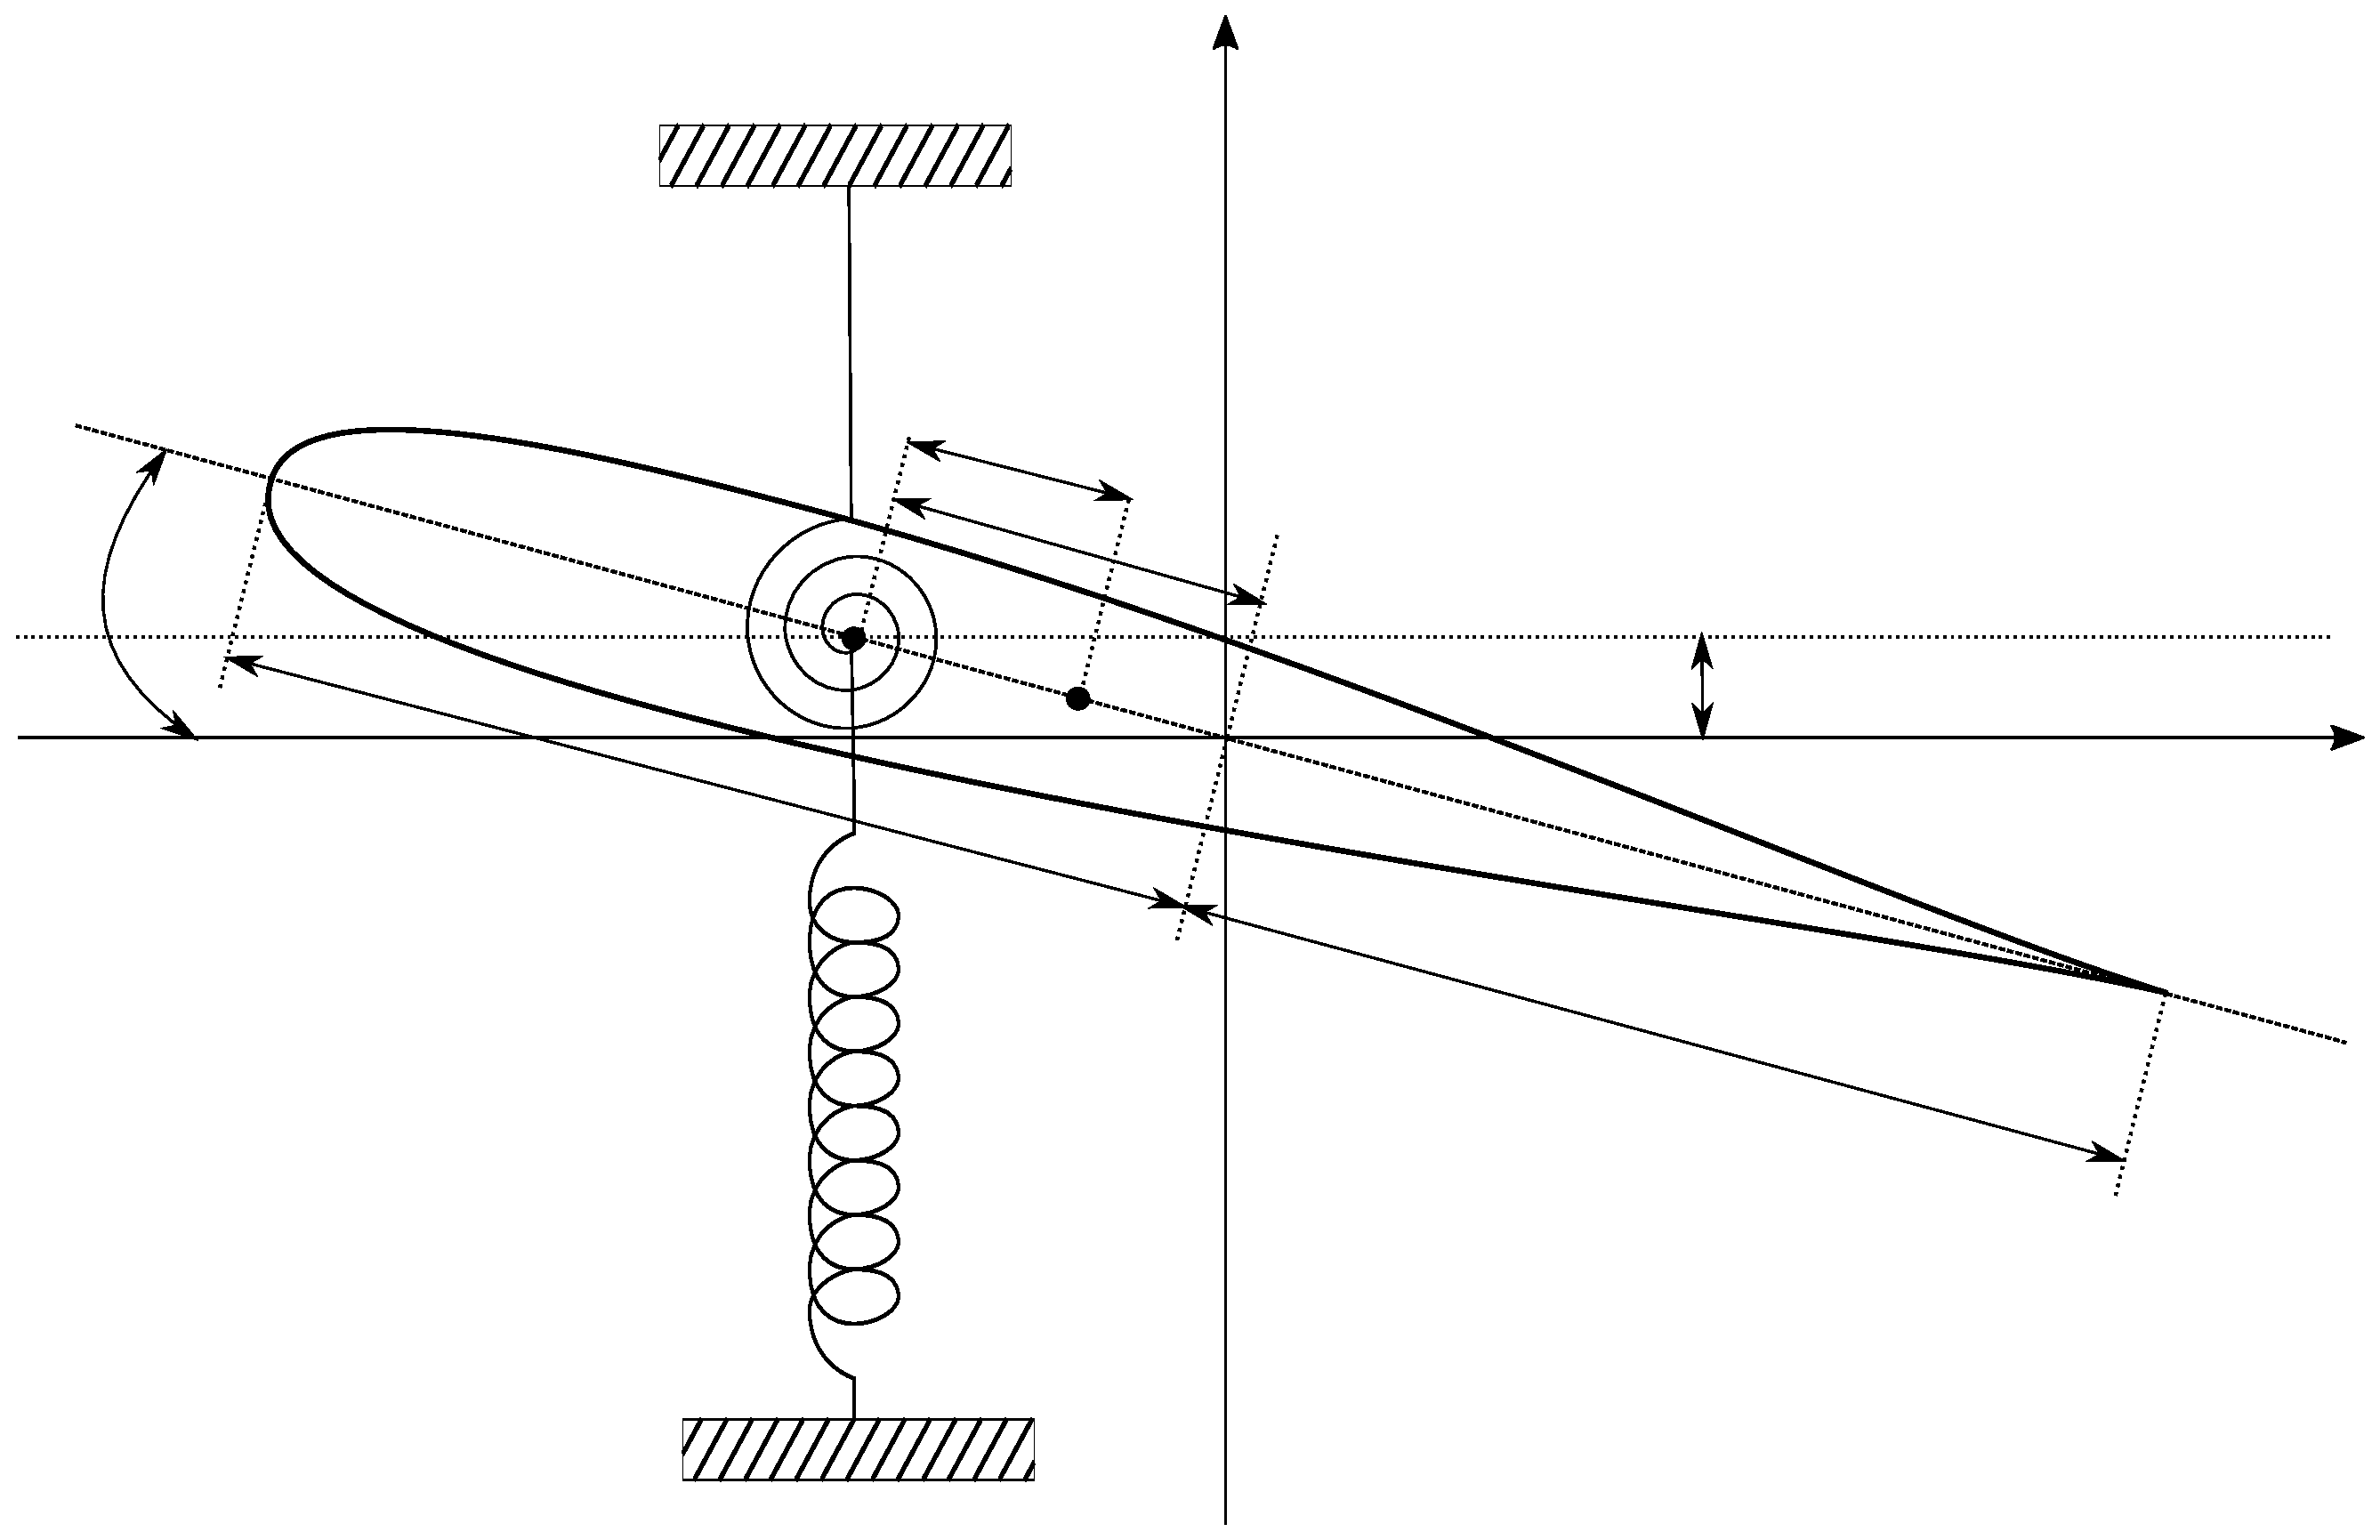
\includegraphics[width=8cm]{flutter_diagram.eps}
  \put(-215,87){$\alpha$}
  \put(-165,65){$b$}
  \put(-70,40){$b$}
  \put(-130,105){$x_{\alpha}$}
  \put(-127,95){$a$}
  \put(-70,78){$h$}
  \caption{Schematic drawing of simplified aeroelastic model.}
  \label{fig:diagram}
\end{figure}

\begin{figure}
  \pgfplotsset{every axis title/.append style={at={(0.5,0.95)}}}
  \begin{tikzpicture}
  \begin{groupplot}[group style={group size=1 by 1,horizontal sep=40pt,every plot/.style={xmin=13,xmax=19,ymin=0,ymax=0.04},xlabels at=edge bottom,vertical sep=30pt},width=12cm,height=7.5cm,xlabel={Wind speed (m/sec)},x label style={at={(0.5,-0.05)}},scatter/classes={%
  		a={mark=*,mark size=2pt,blue},%
  		b={mark=o,mark size=2pt,red}},legend style={at={(0.33,0.95)}},every axis plot/.append style={ultra thick}]

  \nextgroupplot[ylabel={Heave Amplitude (m)},y label style={at={(-0.02,0.5)}}]
          \draw[->] (axis cs:14, 0.014) -- (axis cs:14, 0.005);
          \draw[->] (axis cs:14, 0.016) -- (axis cs:14, 0.018);
          \draw[->] (axis cs:14, 0.035) -- (axis cs:14, 0.02);
          \draw[->] (axis cs:15, 0.012) -- (axis cs:15, 0.005);
          \draw[->] (axis cs:15, 0.015) -- (axis cs:15, 0.02);
          \draw[->] (axis cs:15, 0.035) -- (axis cs:15, 0.023);
          \draw[->] (axis cs:16, 0.010) -- (axis cs:16, 0.005);
          \draw[->] (axis cs:16, 0.013) -- (axis cs:16, 0.022);
          \draw[->] (axis cs:16, 0.035) -- (axis cs:16, 0.026);
          \draw[->] (axis cs:17, 0.0065) -- (axis cs:17, 0.005);
          \draw[->] (axis cs:17, 0.011) -- (axis cs:17, 0.024);
          \draw[->] (axis cs:17, 0.035) -- (axis cs:17, 0.029);
          \draw[->] (axis cs:18, 0.008) -- (axis cs:18, 0.026);
          \draw[->] (axis cs:18, 0.035) -- (axis cs:18, 0.031);
  \addplot [no marks,color=blue]
        table [x=a, y=b, col sep=comma] {./Data/Data_10-2.csv};\label{ps}
  %Here the blue parabloa is defined
  \addplot [no marks,color=red,dashed]
        table [x=a, y=b, col sep=comma] {./Data/Data_10-1.csv};\label{pu}
  \addplot [no marks,color=blue]
        table [x=a, y=c, col sep=comma] {./Data/Data_10-4.csv};
        %Here the blue parabloa is defined
  \addplot [no marks,color=red,dashed]
        table [x=a, y=c, col sep=comma] {./Data/Data_10-3.csv};

  \end{groupplot}
  \end{tikzpicture}
  \centering
\caption{ Bifurcation diagram of unsteady aeroelastic model with physical parameters given in \Tref{t2}. (\ref{ps}) is stable LCO and stable equilibria, (\ref{pu}) is unstable LCO and unstable equilibria. Arrows represents projection of phase portrait near the equilibria and LCO.}
\label{f:TH}
\end{figure}

\section{Control based continuation (CBC)}\label{CBC}

Periodic solution $\vec{u}(t)$, where $\dot{\vec{u}}(t) =\vec{F}(\vec{u}(t),\vec{\lambda})$ with period $T$ of \Eref{eq:gs}, can be tracked via numerical continuation by defining zero problem as

\begin{align}\label{eq:zp2}
  \begin{split}
 \vec{u}(T)-\vec{u}(0)&=0,\\
   \int_{0}^{T} <\dot {\vec{u}}, \vec{u}> dt&=0,
\end{split}
\end{align}

\noindent where $<\cdot,\cdot>$ denotes inner product of vector. This zero problem has a boundary value problem of periodic motion and phase condition to parametrize the family of periodic orbit as element and the zero problem is solved by suitable methods such as newton methods at each $\lambda$.


Continuation of a periodic solution in the experiment needs a different approach with numerical continuation. First, the unstable periodic solution should be stabilized by feedback control. Scalar control force $\Gamma(t)$ with proportional derivative control can be expressed as

\begin{align}
  \Gamma(t)=K_p(x^*(t)-x(t))+K_d(\dot x^*(t)-\dot x(t)),
\end{align}

\noindent where $x(t)$ is a scalar output of the system (measured signal), $x^*(t)$ is a scalar control target, $K_p$ is the proportional control gain, and $K_d$ is the derivative control gain. Measuring unstable periodic solution is achieving a noninvasive control which means $\Gamma(t)=0$. Then, control target $x^*(t)$ is identical to unstable periodic if $K_p$, $K_d$ are selected appropriately to stabilize the unstable periodic solution of the uncontrolled system.

$x^*(t)$ that makes the controller noninvasive can be computed from the experiment by solving zero problem defined by input-output map $x^*(t)-x(t)=0$. For instance, input-output map can be discretized by projecting $x^*(t)$ and $x(t)$ to Fourier series of first $2q+1$ modes for the harmonically forced vibrations as

\begin{align}\label{eq:dis}
  \begin{split}
  x(t)=&A_0/2+  \sum_{j=1}^{q} A_j \cos (j\omega t)+B_j \sin (j\omega t),\\
  x^*(t)=&A_0^*/2+  \sum_{j=1}^{q} A^*_j \cos (j\omega t)+B^*_j \sin (j\omega t).
\end{split}
\end{align}

\noindent This expression gives discretized fixed point problem with $2q+1$ equations as

\begin{align}\label{eq:zp}
  \begin{split}
  A_j=&A^*_j \; \textrm{for} \; j=0,1,\ldots,q\\
  B_j=&B^*_j,\; \textrm{for} \; j=1,2,\ldots,q
\end{split}
\end{align}

\noindent \Eref{eq:zp} allows us to define zero problem for multidimensional systems even if we are using scalar input $x^*(t)$ and output $x(t)$ when the feedback control is stabilizing the response. Fixed point problem of CBC can be solved using any zero problem-solving methods such as Newton-like methods \cite{schilder2015experimental} or Picard iteration \cite{barton2013systematic}. Note that CBC is equation-free method and in fact, it can be used to build a mathematical model which will be discussed in the later section.

However, stabilizing unstable LCO with CBC is not simple because of the complexity of the input-output map of forced Hopf bifurcation. Zero problem to be solved in the experiment cannot be defined if we use a typical CBC scheme that discretizes periodic orbit with first $2q+1$ fourier coefficients. We will discuss the input-output map of CBC for Hopf bifurcation and define a zero problem in the next section.

\section{Stablizing control near the Hopf bifurcation}\label{SNH}

Simplifying the dynamical system using normal form is the most popular way to study the bifurcation problem analytically. There are numerous tools to derive normal form, for example, center manifold reduction, Liapunov-Shmidt reduction and method of multiple scales. In this research, we focus on studying controlled and uncontrolled dynamics near the Hopf bifurcation via center manifold reduction, near-identity transformation, time, and control parameter rescaling to discuss the stabilizability of the controller. Simplified dynamics of CBC applied to a dynamical system with Hopf bifurcation provides the basis of the developed CBC scheme of this research.

\subsection{Hopf bifurcation and the normal form}\label{SNF}

Simplifying the dynamical system is a powerful tool to understand the dynamics of the Hopf bifurcation and the CBC. First, \Eref{eq:gs} should be transformed to a partitioned system at \(\lambda=0\) by transforming the linearization of \(\vec{F}\) to Jordan normal form as
\begin{align}\label{eq:2}
  \begin{split}
    \dot{\vec{x}} =\vec{J}_\textrm{c} \vec{x} + \vec{f}(\vec{x},\vec{y},\lambda)\\
    \dot{\vec{y}} =\vec{J}_\textrm{s} \vec{y} +\vec{g}(\vec{x},\vec{y},\lambda)
  \end{split}
\end{align}
where $\vec{x}=[x;\bar{x}]\in \complex^2$ is center subspace with associated Jordan matrix $\vec{J}_\textrm{c}$ having diagonal term $\pm\textrm{i}$ and $\vec{y}\in \complex^{n-2}$ is stable subspace with it's associated Jordan matrix $\vec{J}_\textrm{s}$ of Jacobian of $\vec{F}(\vec{z})$ at $\vec{z}=0$.
$\vec{f}$ and $\vec{g}$ are functions with $\vec{f}(0,0)=0$, $D\vec{f}(0,0)=0$ and $\vec{g}(0,0)=0$, $D\vec{g}(0,0)=0$. Centermanifold exists for dynamical system \Eref{eq:2} for small  $\|\vec{x}\|$ which is invariant under the action of dynamical system \cite{carr2012applications}. Note that eigenvalues corresponding to center subspace is assumed $\pm\textrm{i}$ for simplicity. To reduce the order of dynamics of Hopf bifurcation, we include $\dot\lambda=0$ to \Eref{eq:2} and analyze the family of center manifolds, locally represented by small $\|\lambda\|$  \cite{kuznetsov2013elements}. Power series of centermanifold $\vec{H}(\vec{x},\lambda)$ can be computed recursively by solving
\begin{align}\label{eq:3}
    D\vec{H}({\vec{\hat{x})}}(\vec{\hat{J}}_\textrm{c}\vec{\hat{x}}+\vec{f}(\vec{\hat{x}},\vec{H}(\vec{\hat{x}}))) =\vec{J}_\textrm{s} \vec{H}(\vec{\hat{x}})-\vec{g}(\vec{\hat{x}},\vec{H}(\vec{\hat {x}}))
\end{align}
at each order of power series, where \(\vec{\hat{x}}=[\lambda;\vec{x}]\) and \(\vec{\hat{J}}_c\) is the extended Jordan matrix which zero eigenvalue is added to \(\vec{J}_\textrm{c}\) \cite{bi1999symbolic}. Then, we can compute the reduced dynamics on the centermanifold as a power series which will have a form as
\begin{align}\label{eq:4}
  \begin{split}
    {}&\dot{x} =\textrm{i} x+\sum_k f_k(x,\bar{x},\lambda)\\
    ,\textrm{where} \; & f_k=\sum_{j+l+m=k}(\vec{a}_{1jlm}+\textrm{i}\vec{a}_{2jlm})x^j\bar{x}^l\lambda^m.
  \end{split}
\end{align}
Note that in \Eref{eq:4}, \(\lambda=[\lambda_1;\lambda_2;\ldots;\lambda_m]\) and \(\lambda^m\) denotes \(\lambda_1^{m_1}\lambda_2^{m_2}\cdots\lambda_m^{m_m}\) satisfying \(\sum_i m_i = m\) with \(\vec{a}_{1jlm}=[a_{1jlm_1};a_{1jlm_2};\ldots;a_{1jlm_m}]\).

Recently, researchers have worked extensively to develop an efficient simplest normal form of Hopf bifurcation using computer algebra \cite{algaba1998hypernormal,yu1998computation}. Simplest normal form (SNF), simplest means that the number of terms retained at each order of is minimized, is one of the most effective ways to derive the normal form from the nonlinear differential equation defined on center manifold. Moreover, we can parametrize amplitude of LCO by parameters of the original coordinate system if we use SNF. Unlike the dynamical system without control parameters, SNF cannot be computed using only near identity transformation. P.Yu \cite{yu2002simplest} proved time and parameter rescaling is essential additional to near identity transformation and developed a recursive formula to compute SNF up to k-th order; however, we limit our attention up to third order. SNF can be expressed as
\begin{align}\label{eq:5}
  \begin{split}
    &\frac{du}{d\tau}=(\vec{\alpha}_1+\textrm{i}\vec{\beta}_1)\nu u+(\vec{\alpha}_2+\textrm{i}\vec{\beta}_2) u^2 \bar{u}+\textrm{i}\sum_k g_k(u,\bar{u}),\\
    \textrm{where} \;  &g_k(u,\bar{u})=(b_{1k}+\textrm{i}b_{2k})u^{\frac{k+1}{2}}\bar{u}^{\frac{k-1}{2}}, \; \textrm{for odd integer} \;k.
  \end{split}
\end{align}
Here, \(\vec{u}=[u,\bar{u}]\) and equation of complex conjugate variable \(\bar{u}\) is neglected. \(u\),\(\tau\) and \(\nu\) are transformed from \(x\),\(t\) and \(\lambda\) by following near identity transformation
\(x=h(u,\bar{u},\nu))=u+\sum_k h_k(u,\bar{u},\nu)\), time rescailing \(t=T(u,\bar{u},\nu,\tau)\) and parameter rescailing \(\lambda=p(\nu)\),
\begin{align}\label{eq:6}
  \begin{split}
    h_k &=\sum_{j+l+m=k}(c_{ijkm}+\textrm{i}c_{2jlm}u^j\bar{u}^l \nu^m),\\
    t &=\Big(1+\sum_{k=1}\sum_{j+m=k}t_{jm}[(u+\bar{u})]^j\nu^m\Big)\tau,\\
    \lambda &=\nu+\sum_{j=2}p_j \nu^j.
  \end{split}
\end{align}
Coefficients of \Eref{eq:6} can be computed recursively \cite{yu2002simplest} by eliminating noncritical terms of \Eref{eq:4}, SNF of Hopf bifurcation is derived with coefficients of original coordinate as

\begin{align}\label{eq:9}
&\frac{du}{d\tau}=\textrm{i}u+\vec{a}_{1101}\nu u+(a_{1210}-a_{1200}a_{2110}-a_{2200}a_{1110})u^2\bar u+\textrm{i}\sum_{m=1}b_{2(2m+1)}u^{m+1}u^m.
\end{align}

\noindent This can be expressed in a more simpler form by transforming to polar coordinates,

\begin{align}\label{eq:10}
\begin{split}
\frac{dR}{d\tau}=&\vec{a}_{1101}\nu R+(a_{1210}-a_{1200}a_{2110}-a_{2200}a_{1110})R^3\\
\frac{d\theta}{d\tau}=&1+b_{23}R^2,
\end{split}
\end{align}

\noindent where $u=Re^{\textrm{i} \theta}$, $\bar u=Re^{-\textrm{i} \theta}$. The stability of limit cycle can be analyzed from \Eref{eq:10}; for instance, Hopf bifurcation is supercritical if \(a_{1210}-a_{1200}a_{2110}-a_{2200}a_{1110}<0\) and subcritical if \(a_{1210}-a_{1200}a_{2110}-a_{2200}a_{1110}>0\).


\subsection{Stabilizability of the controller}

We will consider linear proportional derivative control acting on a single coordinate vector which will be the most simple case to setup a nonlinear dynamic experiment in various applications. Let the equation of motion of autonomous dynamical system that has  generic subcritical Hopf bifurcation at $\mu=0$ be

\begin{align}\label{eq:0}
    \dot{\vec{z}} =\vec{G}(\vec{z},\vec{\mu}).
\end{align}

\noindent where $\mu\in \real$ is an unfolding parameter of uncontrolled system, and $z_{j+1}=\dot z_j$ for all odd $j$. To stabilize the unstable periodic orbit near the Hopf bifurcation point, we add a proportional derivative feed-back control to \Eref{eq:0}. Let us assume that the control force is applied in the direction of the one principle coordinates to \Eref{eq:0} as

\begin{align}\label{eq:11}
    \dot{\vec{z}} =\vec{G}(\vec{z},\vec{\mu})+\vec{e}_{j+1}(K_p(z^*(t)-z_j)+K_d(\dot z^*(t)-z_{j+1})),
\end{align}

\noindent where $\mu\in \real$ is an control parameter of uncontroled system, $\vec{e}_{j+1}$ is $j+1$ th standard basis, $z_{j}$, $z_{j+1}$ are monitored signal for the control, and $z^*(t)$  is the time-periodic control target. We will show the controlled system can be simplified to forced Hopf bifurcation where the single harmonic forcing is added to a SNF of the unforced equation under a certain assumption. First, we analyze autonomous term of \Eref{eq:11} by dropping off the time-periodic forcing $\vec{e}_{j+1}(K_p(z^*(t))+K_d(\dot z^*(t)))$ as

\begin{align}\label{eq:12}
    \dot{\vec{z}} =\vec{G}(\vec{z},\vec{\mu})-\vec{e}_{j+1}(K_p z_j+K_d z_{j+1}).
\end{align}

\noindent \Eref{eq:12} can be written in the form of \Eref{eq:gs} by

\begin{align}\label{eq:13}
\begin{split}
  F({\vec{z}})=&\vec{G}(\vec{z},\vec{\mu})-\vec{e}_{j+1}(K_pz_j+K_d z_{j+1})\\
  \lambda=&[\mu,K_p,K_d]^T.
\end{split}
\end{align}

\noindent As explained in \Ssref{SNF}, we can derive the reduced dynamics on center manifold of \Eref{eq:13} and compute SNF using nonlinear transformation between center subspace of origianl coordinates $[x,\bar x]^T$ and normal form coordinates $[u,\bar u]^T$ and rescailing time and control parameters.

Now, stabilizability of unstable limit cycle of the uncontroled system can be studied from normal form of \Eref{eq:12} at $\lambda=\lambda_1=[\mu,0,0]^T$. Unstable limit cycle ($[u_1(\tau),\bar u_1(\tau)]^T$) is a nonzero fixed point of SNF \Eref{eq:10} and expressed in normal form coordinates $[u,\bar u]^T$ as

\begin{align}\label{eq:14}
  \begin{split}
      u_1(\tau)=&R_1e^{\textrm{i}\omega_1 \tau},\\
      \bar u_1(\tau)=&R_1e^{-\textrm{i}\omega_1 \tau},
    \end{split}
\end{align}

\noindent where $R_1$ is the amplitude and $\omega_1$ is frequency of the limit cycle in rescailed time. If we define homeomorphism($\Psi_1:\complex\times\complex\rightarrow\complex\times\complex$) between the original coordinates $[x,\bar x]^T$ and normal form coordinates $[u,\bar u]^T$ at $\lambda=\lambda_1$ as

\begin{align}\label{eq:15}
    [x,\bar x]^T=\Psi_1(u,\bar u)=&[h(u,\bar u,\nu_1),\bar h(u,\bar u,\nu_1)]^T,
\end{align}

\noindent  where $\nu_1=p^{-1}(\lambda_1)$ is control parameter reparametrization in the coordinates of the normal form with $p(0)=0$. Limit cycle \Eref{eq:14} in original coordinates $x^*(t)$ can be computed from

\begin{align}\label{eq:16}
    [x^*(\tau),\bar {x^*}(\tau)]^T=\Psi_1(R_1e^{\textrm{i}\omega_1 \tau},R_1e^{-\textrm{i}\omega_1 \tau}).
\end{align}

\noindent If we define \textbf{Noninvasive periodic solution} as a periodic solution of \Eref{eq:11} where control force $\vec{e}_{j+1}(K_p(z^*(t)-z_j)+K_d(\dot z^*(t)-z_{j+1}))$ is zero, noninvasive periodic solution of \Eref{eq:11} is solution of \Eref{eq:0} since $\vec{e}_{j+1}(K_p(z^*(t)-z_j)+K_d(\dot z^*(t)-z_{j+1}))=0$. Moreover, by assuming $\| \lambda \|$ is small enough to say small amplitude periodic solution of \Eref{eq:13} is on the center manifold, we can derive the following lemma which relates the control target and the noninvasive periodic solution.

\begin{lemma}\label{l1}
$\vec{z}(t)=\vec{\Sigma}[x^*,\bar {x^*},\vec H(x^*,\bar {x^*},\lambda)]^T$ is a noninvasive periodic solution for \Eref{eq:11} if and only if $z^*(t)=\pi_j (\vec{\Sigma}[x^*,\bar {x^*},\vec H(x^*,\bar {x^*},\lambda)]^T)$,
where $\vec{\Sigma}$ is a coordinate transformation matrix to jordan normal matrix $\vec{J}$ satisfying $\vec{J}=\Sigma^{-1}\vec{F}_\vec{z}(0,\lambda) \Sigma$ at $\lambda=0$, and $\pi_j$ is a scalar projection to j-th principle coordinate.
\end{lemma}

\begin{proof}
If $z^*(t)=\pi_j (\vec{\Sigma}[x^*,\bar {x^*},\vec H(x^*,\bar {x^*},\lambda)]^T)$, by inserting $\vec z(t)=\vec{\Sigma}[x^*,\bar {x^*},\vec H(x^*,\bar {x^*},\lambda)]^T$ to \Eref{eq:11}, we have $\vec{G}(\vec{z},\mu)=0$ and the control force is zero. For the only if part, lets assume $z(t)=\vec{\Sigma}[x^*,\bar {x^*},\vec H(x^*,\bar {x^*},\lambda)]^T$ is a noninvasive periodic solution. Then, $z^*(t)=\pi_j (\vec{\Sigma}[x^*,\bar {x^*},\vec H(x^*,\bar {x^*},\lambda)]^T)$ since the solution is noninvasive.
\end{proof}

\noindent Let $\lambda_2=[\mu,K_p,K_d]^T$ and stability of the noninvasive periodic solution $\vec{z}(t)=\vec{\Sigma}[x^*,\bar {x^*},\vec H(x^*,\bar {x^*},\lambda)]^T$ with control target $z^*(t)=\pi_j (\vec{\Sigma}[x^*,\bar {x^*},\vec H(x^*,\bar {x^*},\lambda)]^T$  at $\lambda=\lambda_2$ will be analyzed. We make the following assumption on the coefficients of $h(u,\bar u,\nu)$ and response $\vec{z}(t)$ to develop a scheme that is practically applicable in experiments.

\begin{assumption}\label{a1}
For $\lambda=\lambda_1$ and $\lambda=\lambda_2$, near identity transformation in \Eref{eq:6} $c_{1jlm}$, $c_{2jlm}$ is sufficiently small, and therefore neglectable for $j+j+m\geq 2$, i.e., $u \approx x$. Also, amplitude of LCO is small enough to say $\tau \approx t$ and $\vec H(x^*,\bar {x^*},\lambda) \approx 0$.
\end{assumption}

\noindent  Under \asref{a1}, periodic solutions in the normal form will be transformed into a single harmonic oscillator in the original coordinates. Therefore, limit cycle in original coordinates $x^*(t)$ and control target  $z^*(t)$ can be expressed as a single harmonic oscillator with small amplitude by using the result of \Lref{l1}. Now, our problem to be solved is Hopf bifurcation with single harmonic forcing. The normal form of forced Hopf bifurcation for small amplitude bounded solution is equivalent to adding force in the direction of the center subspace to the autonomous Hopf normal form \cite{golubitsky2012feed,elphick1987normal}. Therefore, by letting $\epsilon$ as an amplitude of periodic forcing which is appropriately rescailed by projecting $\vec{e}_{j+1}(K_p(z^*(t))+K_d(\dot z^*(t)))$ to the center subspace, normal form of \Eref{eq:11} at $\lambda=\lambda_2$ can be derived as

\begin{align}\label{eq:18}
  \frac{du}{dt}=(\alpha_1+\textrm{i}\beta_1)u+(\alpha_2+\textrm{i}\beta_2)u^2\bar u+\epsilon e^{\textrm{i}\omega_1 t},
\end{align}

\noindent where coefficients $\alpha_1$, $\alpha_2$, $\beta_1$, and $\beta_2$ can be computed from \Eref{eq:9} using the coefficients of reduced dynamics at the centermanifold at $\lambda=\lambda_2$. Stabilizability of the controller can be anlyzed by the stability of the noninvasive periodic solution of \Eref{eq:18} $u=u_2(t)$. Under \asref{a1}, $u_2(t)=R_1e^{\textrm{i}\omega_1 t}$, and stability condition of noninvasive periodic solution can be derived as following lemma.

\begin{lemma}\label{t1}
Noninvasive periodic solution $u_2(t)$ is stable if the amplitude of the noninvasive periodic solution $R_1$ satisfies
\begin{align}\label{eq:20}
3(\alpha_2^2+\beta_2^2)R_1^3+4(\alpha_1+\beta_2(\beta_1-\omega_1))R_1+(\alpha_1^2+(\beta_1-\omega_2)^2)<0.
\end{align}
\end{lemma}

\begin{proof}
If we look \Eref{eq:18} in the rotating coordinates defined by

\begin{align}\label{eq:21}
  v=ue^{\textrm{i}\omega_1 t},
\end{align}

\noindent The dynamical system becomes autonomous,

\begin{align}\label{eq:22}
  \dot v=(\alpha_1+\textrm{i}(\beta_1-\omega_1))v+(\alpha_2+\textrm{i}\beta_2)v^2\bar{v}+\epsilon.
\end{align}

\noindent $v$ satisfying $\dot v=0$ is a phase-locked periodic solution with the forcing of \Eref{eq:18}. We obtain algebraic equation by setting $\dot v=0$ and $R=|v|$,

\begin{align}\label{eq:23}
  ((\alpha_1+\alpha_2R^2)+\textrm{i}((\beta_1-\omega_1)+\beta_2 R^2)))v=-\epsilon.
\end{align}

\noindent $P(R)$, where the zeros of $P(R)$ is phase-locked periodic solutions of \Eref{eq:18}, can be derived by taking norm square of both side of \Eref{eq:23} as

\begin{align}\label{eq:24}
  P(R)=(\alpha_2^2+\beta_2^2)R^6+2(\alpha_1+\beta_2(\beta_1-\omega_1))R^4+(\alpha_1^2+(\beta_1+\omega_1)^2)R^2-\epsilon^2=0.
\end{align}

\noindent Since the noninvasive periodic solution is phase-locked solution of \Eref{eq:18} at $R=R_1$ which is a non-zero fixed point of P(R). Stability of the noninvasive periodic solution can be analyzed from the stability of this fixed point.Therefore, dividing $P_R(R_1)$ by $2R_1^2$, we arrive to the stability condition of the noninvasive periodic solution.
\end{proof}

\noindent The controller is able to stabilize the unstable LCO of the uncontrolled system if the noninvasive periodic solution is stable. For CBC experiments, finding noninvasive control target remains as a problem even if the controller is stabilizable. This will be discussed in the next subsection.

\subsection{Scheme for finding noninvasive periodic solution}\label{FNP}

In many nonlinear dynamic experiments, information about the dynamical system is not given; therefore, noninvasive periodic solution and stabilizability of the control cannot be determined from the equation as in \Sref{SNF}. We will discuss effective scheme to find noninvasive periodic solutions near the Hopf bifurcation in this subsection.

Phase-locked response with the forcing should be tracked from the response of forced Hopf bifurcation, see \cite{zhang2011periodically,wiser2015bifurcations} for detailed bifurcation diagram, to find the noninvasive periodic solution. However, solutions of \Eref{eq:20} are not necessarily to be in phase with forcing frequency. For example, if we set rotating coordinates of \Eref{eq:21} $v=ue^{\textrm{i}(\omega_2 \tau-\theta)}$, where $\theta$ is an arbitrary phase shift, we can rewrite \Eref{eq:18}
as

\begin{align}\label{eq:ps}
\dot v=(\alpha_1+\textrm{i}\beta_1)v+(\alpha_2+\textrm{i}\beta_2)v^2 \bar v+\epsilon e^{\textrm{i}\theta}.
\end{align}

\noindent A stationary solution of \Eref{eq:ps} with arbitrary phase shift $\theta$ is also a periodic response of the controlled system. This phase shift of the response and control target depends on initial condition, which is uncontrollable. Therefore, it makes the problem much simpler if we can force the response to be in phase with a control target to determine the noninvasive periodic solution.

We use a phase plane based CBC (PP-CBC) to achieve phase locking between target coefficients $z^*(t)$ with the response in \Eref{eq:11}. This is equivalent to phase-locking between force and response in \Eref{eq:20}, which was first proposed in \cite{irene}. Monitored signals $z_j$, $z_{j+1}$  are assumed as an analytic signal,

\begin{align}\label{eq:25}
\begin{split}
z_{j}(t)=&A(t)\cos{\phi},\\
z_{j+1}(t)=&-\dot\phi A(t)\sin{\phi}
\end{split}
\end{align}

\noindent where $A(t)$ is the instantaneous amplitude, $\phi$ is the instantaneous phase of the response, $\dot\phi$ is the frequency of the response which is constant if the system is at the steady-state. If we set target coefficient as

\begin{align}\label{eq:26}
z^*(t)=\hat A\cos\Big(\tan^{-1}\Big({\frac{-z_{j+1}(t)}{ \dot \phi z_{j}(t)}}\Big) \Big),
\end{align}

\noindent where $\hat A$ is the amplitude of the control target, phase of the target is locked with the response since single harmonic response is assumed. Specifically, phase is locked by updating $\dot\phi$ every fixed time interval from the measurement and wait until the system reaches the steady-state. This phase-locked condition is equivalent to $\dot v=0$ in \Eref{eq:22} and as a result control target has a form:

\begin{align}\label{eq:tg}
 z^*(t)=\hat A\cos{\phi}.
\end{align}

\noindent Moreover, final steady-state response is the fixed point of $P(R)$ in normal form coordinates if $P_R<0$ with $\epsilon=\epsilon(\hat A)$. Now, zero problem can be derived from input output map which is defined as a one-dimensional function of $\hat A$ by control error $\Xi=\hat A - A(\hat A)$ where $A$ is amplitude of the response in original coordinates. We can say the controller is stabilizable for the noninvasive periodic solution if the sequence of control error $\Xi_k=\hat A_k-A_k$ crosses zero for some $\hat A_k$ with step size $\Delta_k=\hat A_{k+1}-\hat A_{k}$.

Let us say we found a zero-crossing sequence of $\Xi_k$ from the experiment, which means the controller is stabilizable. Then, finding a noninvasive periodic solution is equivalent to finding  $|\Xi_k|<\delta$, where $\delta$ is the zero-tolerance. The noninvasive periodic solution can be found by decreasing the stepsize $|\Delta_k|=|\Delta_{k-1}|/2$ and changing the searching direction whenever $\Xi_k$ crosses zero. This procedure to find zero error $\Xi=0$ can be summarized as \Fref{f:1}.

\begin{figure}
\tikzstyle{decision} = [diamond, draw, fill=blue!20,
    text width=7em, text badly centered, inner sep=0pt, minimum height=3em]
\tikzstyle{decision2} = [diamond, draw, fill=blue!20,
        text width=6em, text badly centered, inner sep=0pt, minimum height=3em]
\tikzstyle{block} = [rectangle, draw, fill=blue!20,
    text width=8em, text centered, rounded corners, minimum height=4em]
\tikzstyle{block2} = [rectangle, draw, fill=blue!20,
        text width=13em, text centered, rounded corners, minimum height=3em]
\tikzstyle{block3} = [rectangle, draw, fill=blue!20,
                text width=8em, text centered, rounded corners, minimum height=3em]
\tikzstyle{block4} = [rectangle, draw, fill=blue!20,
                text width=4em, text centered, rounded corners, minimum height=3em]
\tikzstyle{line} = [draw, -latex']
\tikzstyle{cloud} = [draw, ellipse,fill=red!20, node distance=3cm,
    minimum height=2em]

\begin{center}
\begin{tikzpicture}[node distance = 2cm, auto]
    % Place nodes
    \node [block4] (init) {$\hat A=\hat A_k$};
    \node [block2, below of=init,node distance=1.3cm] (identify) {Wati until system reaches steady state};
    \node [decision2, below of=identify,node distance=1.9cm] (evaluate) {$|\Xi_k|<\delta$};
    \node [block4, left of=evaluate, node distance=4cm] (update) {stop};
    \node [decision, below of=evaluate,node distance=2.7cm] (decide) {$|\Xi_k||\Xi_{k-1}|<0$};
    \node [block3, left of=decide, node distance=4cm] (update2) {$\Delta_k=-\Delta_{k-1}/2$};
    \node [block, below of=decide, node distance=2.3cm] (stop) {$\Delta_k=\Delta_{k-1}$\\ $\hat A_{k+1}=\hat A_k+\Delta_k$ \\$k=k+1$};
    % Draw edges
    \path [line] (init) -- (identify);
    \path [line] (identify) -- (evaluate);
    \path [line] (evaluate) -- node {no} (decide);
    \path [line] (evaluate) -- node [near start] {yes} (update);
    \path [line] (decide) -- node [near start] {yes} (update2);
    \path [line] (decide) -- node {no}(stop);
    \path [line] (update2) |- (stop);
    %  \path [line] (stop.east) [xshift=5em] -- (init.east);
      \path[line] (stop.east) -- (4,-8.2) --(4,0)
   --(init.east);

\end{tikzpicture}
\end{center}
\centering
\caption{Flow chart diagram of finding noninvasive periodic solution}
\label{f:1}
\end{figure}



\section{Experimental example}
In this section, we show scheme developed in \Sref{SNH} can be applied to a mechanical system with Hopf bifurcation. Developed scheme is applied to a flutter rig.


\subsection{Experiment setup}\label{setup}
The experiment was performed on flutter rig with a NACA-0015 wing profile \cite{jacobs1933characteristics}. The profile moves in two degrees of freedom, heave, and pitch. Coil springs are installed to add linear stiffness to the heave and pitch motion, and spring plate is installed to add nonlinearity on the pitch stiffness. Measurements are taken at shaft with digital encoder for pitch and heave motion was measured from laser displacement sensor. Data acquisition and real-time control were performed with Beaglebone Black and real-time controller \cite{rtc2}. Control force was applied to heave motion to stabilize unstable LCO with APS Electro-Seis Shaker and schematics of a configuration of the experiment and picture of the rig is presented in \Fref{f:rig}.

\begin{figure}
  \centering
  \begin{subfigure}[b]{0.6\linewidth}
    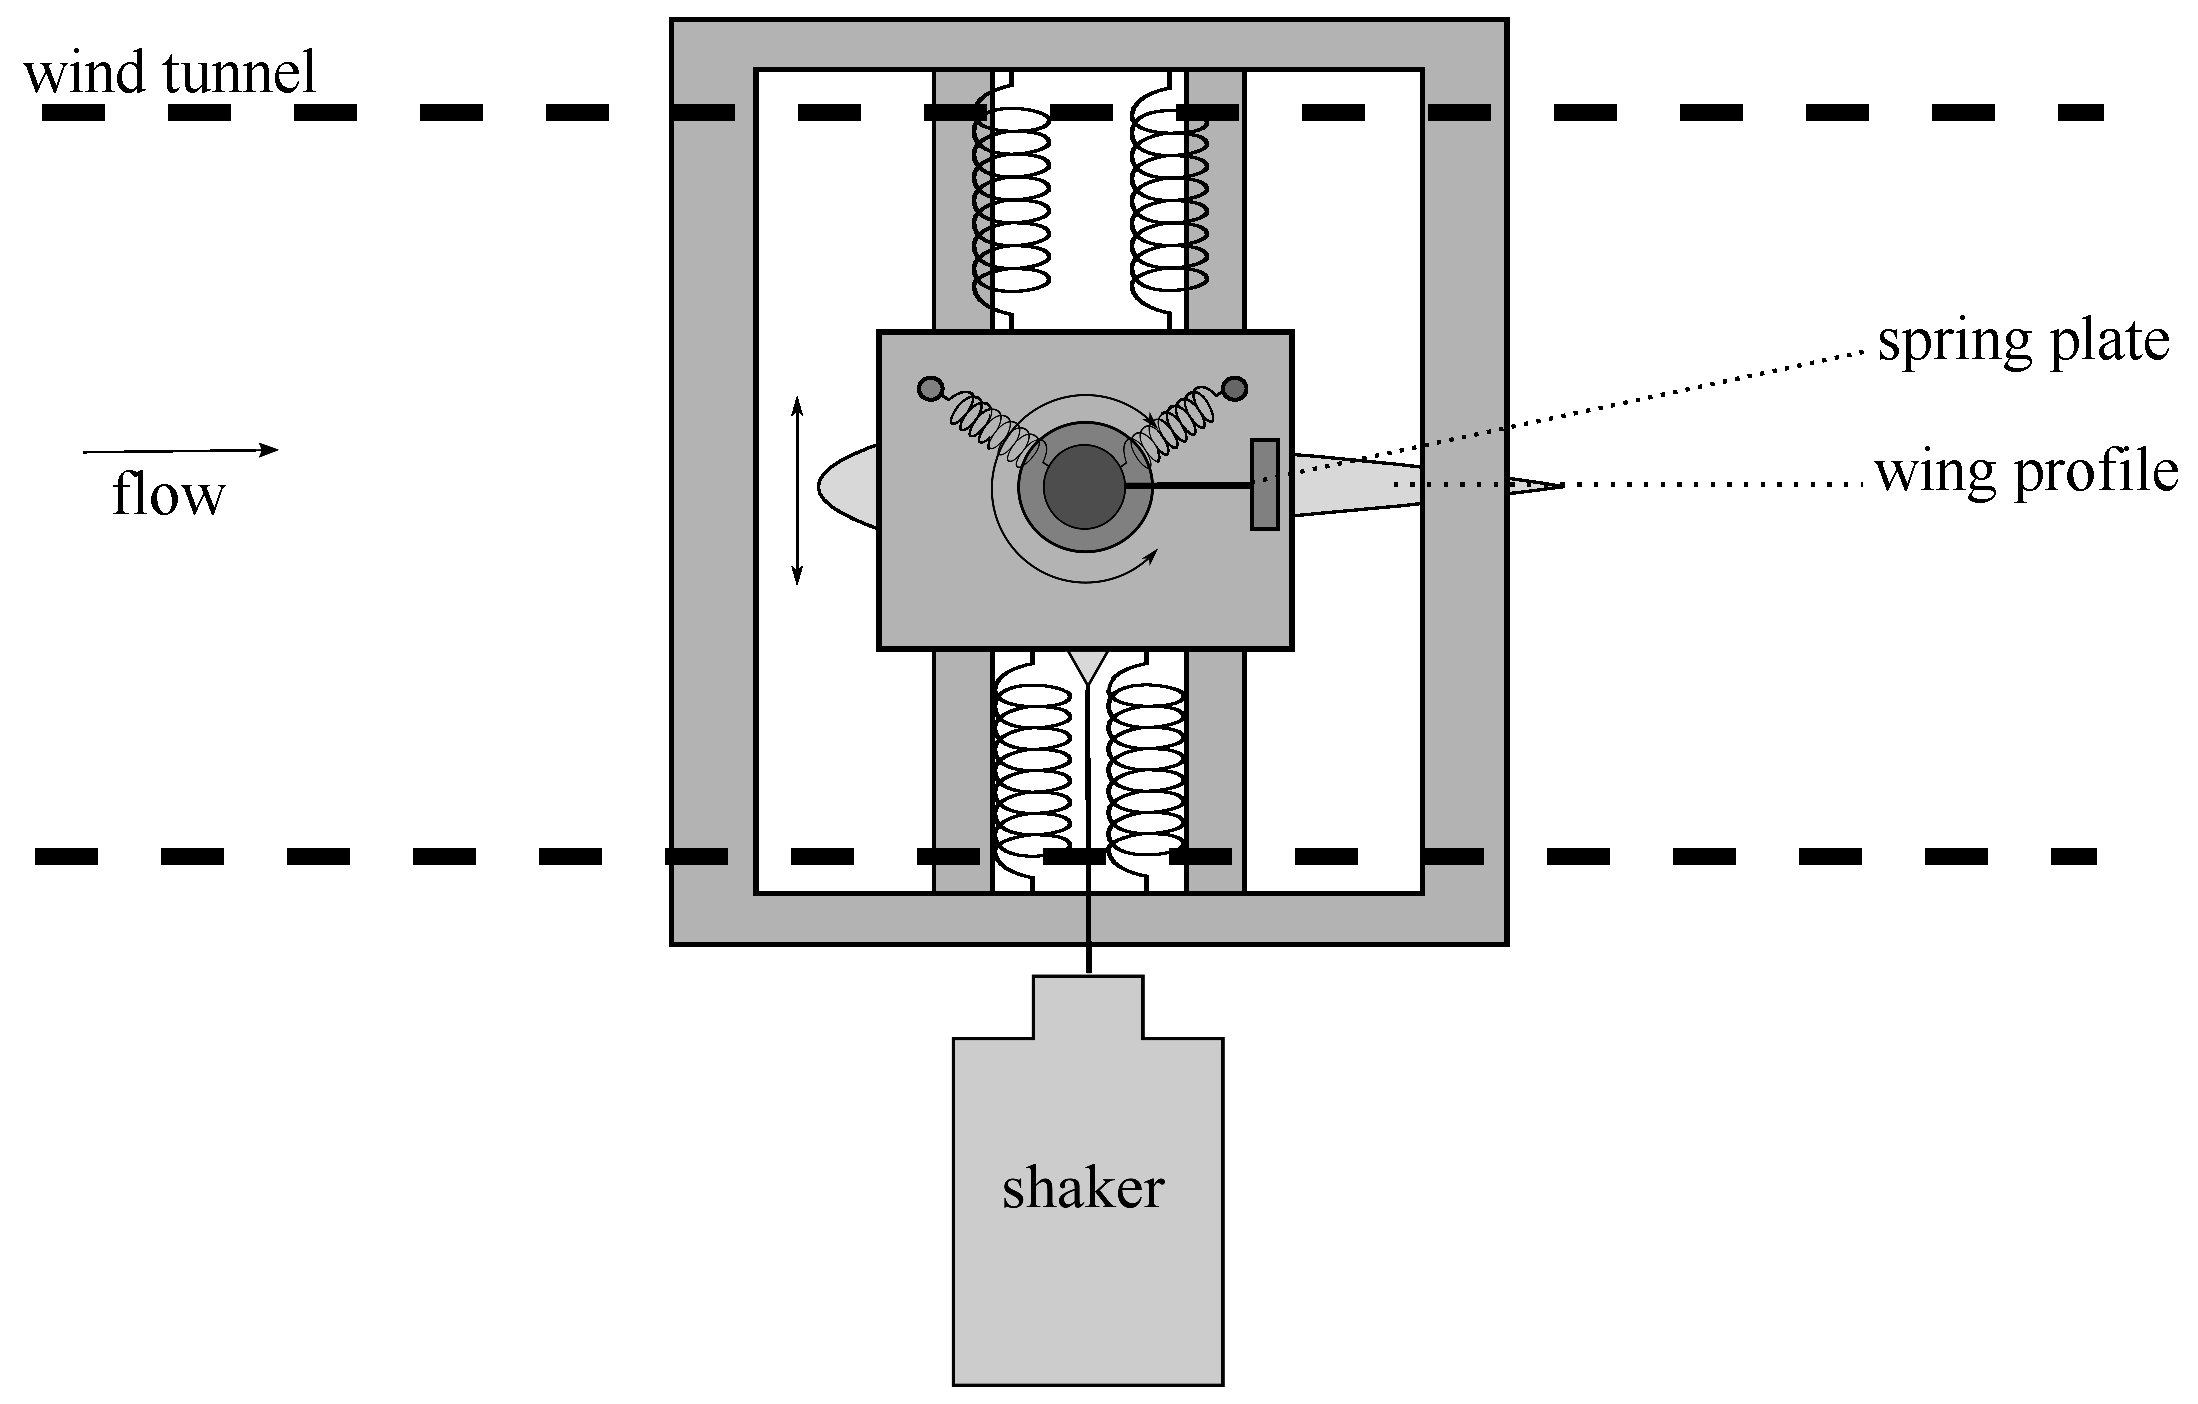
\includegraphics[width=\linewidth]{flutter_rig.eps}
    \caption{Schematic of flutter rig}
  \end{subfigure}
  \begin{subfigure}[b]{0.6\linewidth}
    \includegraphics[width=\linewidth]{rig_pic.png}
    \caption{Picture of flutter rig.}
  \end{subfigure}
  \caption{Schematic drawing and picture of flutter rig.}
  \label{f:rig}
\end{figure}

\subsection{Experiment results}\label{results}

Open-loop tests are performed initially to investigate the dynamics of the system. Below the wind speed approximately 15 $m/sec$, equilibrium is stable and transient response ends with equilibrium state when the large perturbation is applied to equilibrium. However, above the wind speed approximately 15 $m/sec$, transient response ends with stable LCO when even small perturbation is applied to equilibrium. From this observation, we assume that the dynamical system has subcritical Hopf bifurcation and family of LCO has a saddle-node bifurcation at approximately around 15 $m/sec$ which has similar bifurcation diagram with \Fref{f:TH} (b).\\
To stabilize the unstable LCO, we first make multiple measurements at the different amplitude of control target to analyze the stabilizability. \Fref{f:4} (a) shows that the frequency of the phase-locked response with a different amplitude of target coefficient $\hat A$ which shows the frequency of the phase-locked response is parametrized by $\hat A$. Also, We can conclude controller is stabilizable for the unstable LCO if the $\Xi$ crosses zero as \Fref{f:4} (b) for some sequence of $\hat A_k$.


\begin{figure}
  \pgfplotsset{every axis title/.append style={at={(0.5,0.95)}}}
  \begin{tikzpicture}
  \begin{groupplot}[group style={group size=2 by 1,horizontal sep=35pt,xlabels at=edge bottom,vertical sep=30pt},width=7.1cm,height=7.5cm,xlabel={Amplitude of control target ($m$)},ylabel={Heave (m)},x label style={at={(0.5,-0.1)}}]

  \nextgroupplot[title=(a),ylabel={Frequency ($Hz$)},y label style={at={(-0.1,0.5)}},legend style={at={(0.35,0.98)}},ymin=2,ymax=3,every x tick scale label/.style={at={(rel axis cs:0.9,-0.1)},anchor=south west,inner sep=1pt}]

  \addplot [mark=o,color=blue]
        table [x=a, y=c, col sep=comma] {./Data/Data4-1.csv};

  \addplot [mark=triangle,color=red]
        table [x=a, y=c, col sep=comma] {./Data/Data4-2.csv};

  \addplot [mark=square,color=green]
        table [x=a, y=c, col sep=comma] {./Data/Data4-3.csv};
  %Here the blue parabloa is defined
  \nextgroupplot[title=(b),ylabel={Control error $\Xi$ ($m$)},y label style={at={(-0.12,0.5)}},every x tick scale label/.style={at={(rel axis cs:0.9,-0.1)},anchor=south west,inner sep=1pt},ymax=0.005]

  \addplot [mark=o,color=blue]
        table [x=a, y=b, col sep=comma] {./Data/Data4-1.csv};

  \addplot [mark=triangle,color=red]
        table [x=a, y=b, col sep=comma] {./Data/Data4-2.csv};

  \addplot [mark=square,color=green]
        table [x=a, y=b, col sep=comma] {./Data/Data4-3.csv};
  %Here the blue parabloa is defined


  \end{groupplot}

  \end{tikzpicture}
  \centering
\caption{Multiple measurements of frequency and control error of phase-locked periodic solutions at different amplitudes of control target (a) frequency, (b) error.}
\label{f:4}
\end{figure}

\noindent Now, finding a noninvasive point to measure the unstable LCO is equivalent to solving zero problem of $\Xi$, which is a function of $\hat A$. $\Xi$ has two zero points at unstable low amplitude LCO and stable high amplitude LCO. \Fref{f:2} shows the time response of heave response and control target with zero tolerance $\delta=1.8 \: mm$, where we can find input and output is sufficiently identical and phase locking between the control target and the response is accomplished by the real-time controller. We assume the zero tolerance is sufficiently small that the measured unstable and stable LCO has the same amplitude and frequency with the LCO of the uncontrolled system. This can be verified for the stable LCO by switching off the control as shown in \Fref{f:3}, stable LCO maintains it's motion; however, unstable LCO is attracted to stable equilibrium when the controller is turned off.

Noninvasive points were found experimentally to obtain a bifurcation diagram of this dynamical system. Results are presented in \Fref{f:5}, which shows the measured unstable LCO, stable LCO with different wind velocities. \Fref{f:5} (a) has a similar pattern with typical bifurcation diagram of subcritical Hopf bifurcation in \Fref{f:TH}. Experimentally obtained bifurcation diagram contains valuable features of the dynamical system-- saddle-node bifurcation point of LCO, flutter speed, flutter frequency-- which can be used as a tool to verify the mathematical model. Also, measured amplitude and frequency can be used to identify the parameters of the model, which will be discussed in the next section.

In this research, zero problems were not embedded in the pseudo arclength continuation since the wind speed of the wind tunnel was uncontrollable by the real-time controller. However, CBC scheme developed here can be embedded to pseudo arclength continuation if the real-time controller is able to control the control parameter of the Hopf bifurcation.

\begin{figure}
  \pgfplotsset{every axis title/.append style={at={(0.9,0.9)}}}
  \begin{tikzpicture}
  \begin{groupplot}[group style={group size=3 by 2,every plot/.style={xmin=0,xmax=2},xlabels at=edge bottom,ylabels at=edge left,vertical sep=30pt,horizontal sep=20pt,},width=5.0cm,height=3.5cm,xlabel={Time (sec)},ylabel={Heave (m)},y label style={at={(-0.2,0.5)}},x label style={at={(0.5,-0.2)}}]

  \nextgroupplot[title=(a),ymin=-3.5e-2,ymax=3.5e-2]
  \addplot [no marks,color=blue]
        table [x=a, y=b, col sep=comma] {./Data/Data.csv};\label{q1}

  \addplot [no marks,color=red,dashed]
      table [x=a, y=c, col sep=comma] {./Data/Data.csv};\label{q2}
  \nextgroupplot[title=(b),ymin=-3.5e-2,ymax=3.5e-2]
  \addplot [no marks,color=blue]
        table [x=a, y=d, col sep=comma] {./Data/Data.csv};

  \addplot [no marks,color=red,dashed]
      table [x=a, y=e, col sep=comma] {./Data/Data.csv};
  \nextgroupplot[title=(c),ymin=-3.5e-2,ymax=3.5e-2]
  \addplot [no marks,color=blue]
        table [x=a, y=f, col sep=comma] {./Data/Data.csv};

  \addplot [no marks,color=red,dashed]
      table [x=a, y=g, col sep=comma] {./Data/Data.csv};

  \nextgroupplot[title=(d),ymin=-3.5e-2,ymax=3.5e-2]
  \addplot [no marks,color=blue]
        table [x=a, y=h, col sep=comma] {./Data/Data.csv};

  \addplot [no marks,color=red,dashed]
      table [x=a, y=i, col sep=comma] {./Data/Data.csv};
  \nextgroupplot[title=(e),ymin=-3.5e-2,ymax=3.5e-2]
  \addplot [no marks,color=blue]
        table [x=a, y=j, col sep=comma] {./Data/Data.csv};

  \addplot [no marks,color=red,dashed]
      table [x=a, y=k, col sep=comma] {./Data/Data.csv};
  \nextgroupplot[title=(f),ymin=-3.5e-2,ymax=3.5e-2]
  \addplot [no marks,color=blue]
        table [x=a, y=l, col sep=comma] {./Data/Data.csv};

  \addplot [no marks,color=red,dashed]
      table [x=a, y=m, col sep=comma] {./Data/Data.csv};
  \end{groupplot}
  \end{tikzpicture}
  \centering
\caption{(a) Unstable LCO ($U$=14.9 m/sec), (b) Unstable LCO ($U$=15.6 m/sec), (c) Unstable LCO ($U$=16.5 m/sec), (d) Stable LCO ($U$=14.9 m/sec), (e) Stable LCO ($U$=15.6 m/sec), (f) Stable LCO ($U$=16.5 m/sec). (\ref{q1}) is the heave response of the rig, (\ref{q2}) is the control target.}
\label{f:2}
\end{figure}


\begin{figure}
  \pgfplotsset{every axis title/.append style={at={(0.5,0.9)}}}
  \begin{tikzpicture}
  \begin{groupplot}[group style={group size=1 by 2,every plot/.style={xmin=0,xmax=7.0},xlabels at=edge bottom,ylabels at=edge left,vertical sep=30pt},width=13cm,height=3.8cm,xlabel={Time (sec)},ylabel={Heave (m)},y label style={at={(-0.04,0.5)}},x label style={at={(0.5,-0.2)}}]

  \nextgroupplot[title=(a),ymin=-3.5e-2,ymax=3.5e-2]
  \addplot [no marks,color=blue]
        table [x=a, y=b, col sep=comma] {./Data/Data2.csv};


  \nextgroupplot[title=(b),ymin=-1.5e-2,ymax=1.5e-2]
  \addplot [no marks,color=blue]
        table [x=a, y=c, col sep=comma] {./Data/Data2.csv};

  \end{groupplot}
  \end{tikzpicture}
  \centering
\caption{Response of the LCO after the controller truned off at $t=3\;sec$ (a) Stable LCO ($U=\;16.4\;m/sec$), (b) Untable LCO ($U=\;16.4\;m/sec$).}
\label{f:3}
\end{figure}


\begin{figure}
  \pgfplotsset{every axis title/.append style={at={(0.5,0.95)}}}
  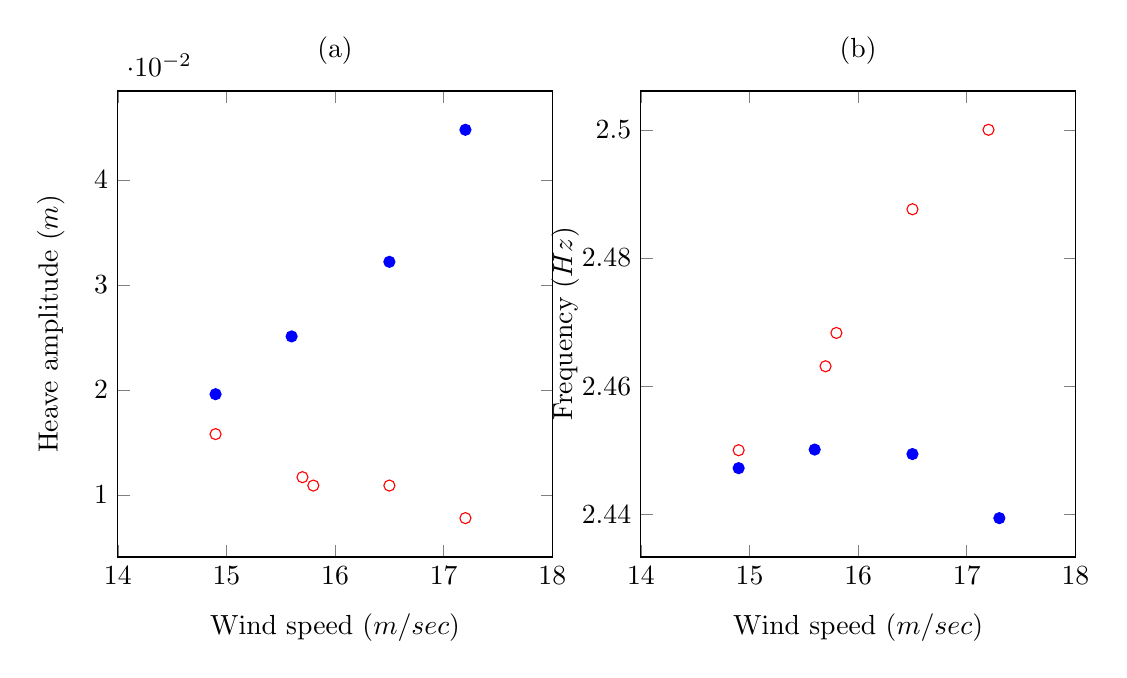
\begin{tikzpicture}
  \begin{groupplot}[group style={group size=2 by 1,horizontal sep=32pt,every plot/.style={xmin=14,xmax=18},xlabels at=edge bottom,vertical sep=30pt},width=7.1cm,height=7.5cm,xlabel={Wind speed ($m/sec$)},ylabel={Heave (m)},x label style={at={(0.5,-0.1)}},	scatter/classes={%
  		a={mark=*,mark size=2pt,blue},%
  		b={mark=o,mark size=2pt,red}},legend style={at={(0.33,0.95)}}]

  \nextgroupplot[title=(a),ylabel={Heave amplitude ($m$)},y label style={at={(-0.1,0.5)}}]
  \addplot [mark=*,only marks,%
		mark size=2pt,blue]
    table {
  x     y
  14.9000    0.0196
  15.6000    0.0251
  16.5000    0.0322
  17.2       0.04477
  	};\label{q3}
    \addplot [mark=o,only marks,%
      mark size=2pt,red]
      table {
    x     y

    14.9000    0.0158
    15.7000    0.0117
    15.8000    0.0109
    16.5000    0.0109
    17.2000    0.0078
      };\label{q4}

  \nextgroupplot[title=(b),ylabel={Frequency ($Hz$)},y label style={at={(-0.12,0.5)}}]
  \addplot [scatter,only marks,%
		scatter src=explicit symbolic]
    table[meta=label] {
  x     y      label
  14.9000    2.4472 a
  15.6000    2.4501 a
  16.5000    2.4494 a
  17.3000    2.4394 a
  14.9000    2.4500 b
  15.7000    2.4631 b
  15.8000    2.4683 b
  16.5000    2.4876 b
  17.2000    2.5000 b
  	};
  \end{groupplot}

  \end{tikzpicture}
  \centering
\caption{CBC results (a) Heave amplitude of LCO ($m$), (b) Frequeny of LCO ($Hz$). (\ref{q3}) is measured stable LCO and (\ref{q4}) is the measured unstable LCO.}
\label{f:5}
\end{figure}


\section{Application of CBC for system identification}
System identification is building a mathematical model from the results of an experiment which can provide valuable physical insights to researchers. We will show CBC can be used to verify the linearized dynamical model and used as a tool to identify the grey-box model \cite{bohlin2006practical} in this section.

\subsection{Physical model for dynamical system}\label{model}
There are many physical models describing flutter; however, we use a simplified 2D model since the wing profile of the flutter rig has a simple shape. To take account of wake effects on the aerodynamic loads, we use unsteady formulation \cite{abdelkefi2013analytical}, which is more accurate compared to quasi-static model \cite{strganac2000identification}. The damping force of the system is assumed as linear viscous damping in both pitch and heave motion, and we assume that spring plate is the only source of nonlinearity in the stiffness. We omit the detailed derivation of unsteady formulation, but a detailed explanation can be found in \cite{abdelkefi2013analytical}. General equation of motion is,

\begin{align}\label{eq:2-1}
\vec{M} \ddot{\vec{p}} + \vec{D} \dot{\vec{p}} +\vec{K_p} \vec{p} + \vec{N}(\vec{p}) =0.
\end{align}

\noindent where

\begin{align}\label{eq:2-2}
\vec{p}=&[h,\alpha,w]^T, \; \vec{N}(\vec{p})=[0,k_{\alpha 2}\alpha^2+k_{\alpha 3}\alpha^3,0]^T,
\end{align}

\begin{align}\label{eq:2-3}
\vec{M}=
\begin{bmatrix}
    m_T+\pi \rho b^2       & m x_\alpha b-a\pi\rho b^3 & 0 \\
    m x_\alpha b-a\pi\rho b^3       & I_\alpha+\pi(1/8+a^2)\rho b^4 & 0 \\
    0       & 0 & 1
\end{bmatrix},
\end{align}

\begin{align}\label{eq:2-4}
\vec D=
\begin{bmatrix}
      c_h+\pi \rho b U        & (1+(1/2-a))\pi b^2 U & 2 \pi U^2 b (c_1c_2+c_3c_4) \\
      -\pi (a+1/2)\rho b^2        & c_\alpha+(1/4-a^2)\pi rho b^3 U & -2 \pi rho b^2 U^2 (a+1/2)(c_1c_2+c_3c_4) \\
      -1/b       & a-1/2 & (c_2+c_4)U/b
\end{bmatrix},
\end{align}

\begin{align}\label{eq:2-5}
\vec K=
\begin{bmatrix}
      k_h        & \pi \rho b U^2  & 2 \pi U^3 c_2 c_4 (c_1+c_3) \\
      0         & k_\alpha - \pi (1/2+a)\rho b^2 U^2 & -2 \pi rho b U^3 (a+1/2)(c_2c_4(c_1+c_3) \\
      0       & -U/b & c_2 c_4U^2/b^2
\end{bmatrix}.
\end{align}

\noindent $w$ is an additional state variable introduced to express the aerodynamic force. Description of parameters used in \Eref{eq:2-1} -  \Eref{eq:2-5} is presented in \Tref{t1} and schematics of coordinate system of the unsteady formulation is given in \Fref{fig:diagram}.


\begin{table}[!ht]
\caption{Parameters of aeroelastic wing}%%%Table caption goes here
\label{table_example}
\begin{tabular}{ll}%%%The number of columns has to be defined here
\hline
Parameter &Description \\
\hline
$b$ & Wing semi-chord ($m$) \\
$a$ & Position of elastic axis relative to the semi-chord  \\
$\rho$ & Air density ($m$) \\
$m_w$ & Mass of the wing ($kg$) \\
$m_T$ & Mass of wing and support ($kg$) \\
$I_\alpha$ & Moment of inertia of wing about the elastic axis ($kg m^2$) \\
$c_\alpha$ & Linear damping coefficient of pitch motion ($kg m^2/s$) \\
$c_h$ & Linear damping coefficient of pitch motion ($kg/s$) \\
$k_\alpha$ & Linear stiffness in pitch ($N$) \\
$k_{\alpha 2}$ & Square nonlinear stiffness in pitch  ($N$) \\
$k_{\alpha 3}$ & Cubic nonlinear stiffness in pitch ($N$) \\
$k_{h}$ & Linear stiffness in heave ($N$) \\
$x_\alpha$ & Nondimensional distance between center of gravity and elastic axis  \\
\hline
\end{tabular}
\vspace*{-4pt}
\end{table}%%%End of the table

\noindent If we express the equation of motion in state variable $ \vec{z} = [h, \dot h, \alpha, \dot \alpha, w, \dot {w}] ^T $, following form can be obtained as

\begin{align}\label{eq:2-6}
\dot{\vec{z}}= \vec{B}(U)\vec{z}+\vec{N_0}(\vec{z}),
\end{align}

\noindent where $\vec{B}(U)$ is the Jacobian of the equation of motion at the equilibruum ($\vec z=0$) which can be computed by rearraging \Eref{eq:2-1} -  \Eref{eq:2-5} to \Eref{eq:2-6}
, and $\vec{N_0}(\vec{z})$ is the nonlinear part of the equation which can be easilly trasformed from $\vec{N}(\vec{p})$.


\subsection{Parameter identification of the linearized model}\label{linear}

We first show unknown parameters of the linearization of grey-box model can be estimated from the linear system identification method. For small-amplitude response, we can neglect the contribution of nonlinear function $\vec{N_0}$ from \Eref{eq:2-6} and the system can be regarded as a linear function. Linear system parameter identification can be done with various existing methods, wavelet transform \cite{ruzzene1997natural}, frequency-domain methods \cite{pintelon2012system}, and state-space models \cite{ljung2001system}. The state-space model provides a direct connection between measurable physical variables and the measured response, while other methods deal with modal properties. Therefore, we use the state-space model to identify the unknown parameters of the experimental rig from the free decay response at low amplitude without flow ($U=0$). Wing semi- chord $b$, the position of the elastic axis relative to the semi-chord $a$, the mass of the wing $m$, the mass of the total wing structure including support $m_T$
modal frequency of pitch $\omega_a=\sqrt{k_\alpha / I_\alpha}$ , modal frequency of the heave $\omega_h=\sqrt{k_h/m_T}$ , and nondimensional distance between center of gravity and elastic axis $x_\alpha$ are the coefficients that can be easilly measured.
Air density $\rho$ is known value and we set $\theta=[I_\alpha,c_\alpha,c_h,\dot h(0),\dot \alpha(0)]^T$ as unknown parameter vector which is more difficult to measure compared to the known parameters. Note that $\dot h(0)$, $\dot \alpha(0)$ are initial value of unmeasured state variables which are unknown parameters and Jacobian of \Eref{eq:2-6} can be written as a function of unknown parameters $\vec{B}(\theta)$. State-space representation of linearized part of \Eref{eq:2-6} can be represented as a finite difference equation when sampling time is $T_s$ as

\begin{align}\label{eq:2-7}
  \begin{split}
\vec{z}(k+1)=&\vec{A}_{T_s}(\theta)\vec{z}(k),\\
\vec{y}=&\vec{C}\vec{z}+\vec{w},
\end{split}
\end{align}

\noindent where $\vec{C}=diag(1,0,1,0)$ is matrix that relates state variable and measured output $\vec{y}$, $\vec{w}$ is measurement noise, and $\vec{A}_{T_s}$ can be computed as

\begin{align}\label{eq:2-8}
\vec{A}_{T_s}(\theta)=e^{\vec{B}(\theta)T_s}.
\end{align}


\noindent To identify the unknown parameters, we use prediction-error identification methods \cite{ljung2001system}. Prediction error \vec{\hat \epsilon} can be defined as

\begin{align}\label{eq:2-9}
\vec{\hat \epsilon}(k,\theta)=\vec{y}(k)-\hat{\vec{y}}(k|\theta),
\end{align}

\noindent where $\hat{\vec{y}}(k|\theta)$ is predicted response from \Eref{eq:2-7}. Parameters that minimize the prediction error $\hat \theta$ can be estimated by

\begin{align}\label{eq:2-10}
\hat{\theta}=\underset{\theta \in D_m}{\arg\min} \: V_N(\theta,\vec{Z}^N),
\end{align}

\noindent where $D_m$ is vector space of unknown parameters, $V_N$ is the summation of vector norm of filtered prediction error, $N$ is the length of the free-decay data, and $\vec{Z}^N$ is a vector containing all measured signal. See \cite{ljung2001system} for details about the filter and the algorithm. Values of identified parameters and measured parameters are given in \Tref{t2}.

\begin{table}[!ht]
\caption{Values of parameters of linearized model}%%%Table caption goes here
\label{t2}
\begin{tabular}{llll}%%%The number of columns has to be defined here
\hline
Measured Parameter & Value & Identified parameter & Value \\
\hline
$b$ & 0.15  $m$ & $I_{\alpha}$ & 0.1724  $kgm^2$ \\
$a$ & -0.5 & $c_\alpha$ & 0.5628  $kgm^2/s^2$ \\
$\rho$ & 1.204  $kg/m^3$ & $c_h$  & 14.5756  $kg/s$ \\
$k_{h}$ & 3529.4  $N/m$ & $k_\alpha$ & 54.11  $N$ \\
$m_w$ & 5.3  $kg$ & & \\
$m_T$ &  16.9  $kg$ & &  \\
$x_\alpha$ & 0.24 & & \\
\hline
\end{tabular}
\vspace*{-4pt}
\end{table}%%%End of the table

\noindent CBC results can be used to check if the identified linear model captures important bifurcation characteristics such as flutter speed and flutter frequency. The verification of the linearized model can be done by comparing flutter speed and flutter frequency with the CBC results. Under \asref{a1}, the square of LCO amplitude is proportional to the control parameter. Therefore, flutter speed can be estimated from the linear regression of the square of LCO amplitude crosses zero (\Fref{f:6} (a)), and flutter frequency can be estimated from the relation between the control parameter and the frequency of the LCO from \Eref{eq:10} which is a linear function if we truncate the normal form to the third order (\Fref{f:6} (b)).

\begin{figure}
  \pgfplotsset{every axis title/.append style={at={(0.5,0.95)}}}
  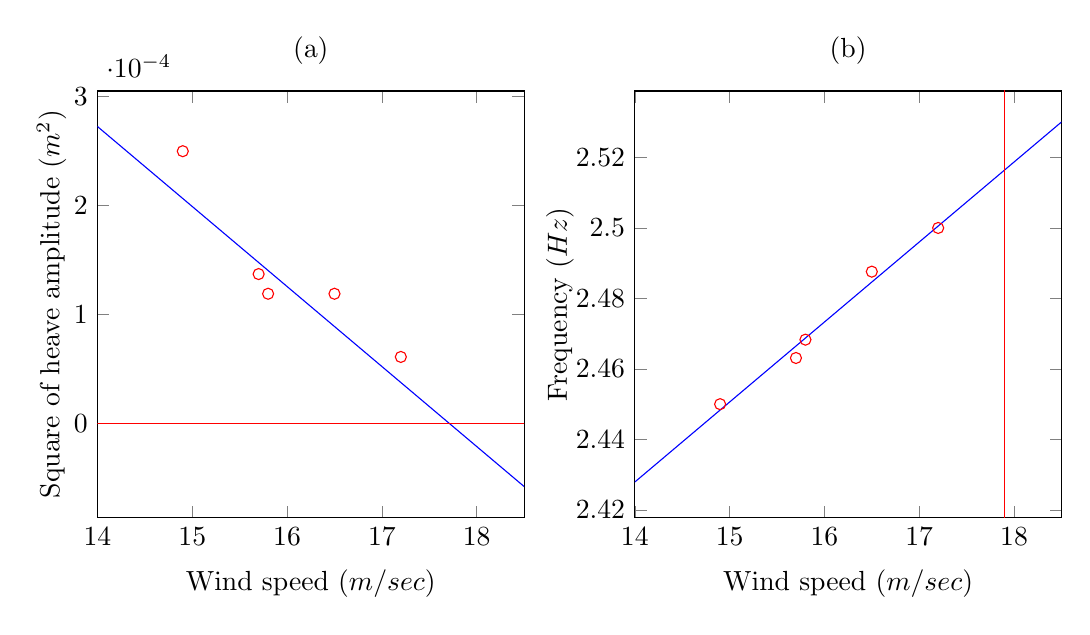
\begin{tikzpicture}
  \begin{groupplot}[group style={group size=2 by 1,horizontal sep=40pt,every plot/.style={xmin=14,xmax=18.5},xlabels at=edge bottom,vertical sep=30pt},width=7cm,height=7cm,xlabel={Wind speed ($m/sec$)},ylabel={Heave (m)},x label style={at={(0.5,-0.1)}}]

  \nextgroupplot[title=(a),ylabel={Square of heave amplitude ($m^2$)},y label style={at={(-0.05,0.5)}}]

  \addplot [
      domain=14:19,
      samples=10,
      color=blue,
  ]
  {-7.3408e-05*x+0.0013};
  \draw [red] (axis cs:13,0)--(axis cs:19,0);
  %Here the blue parabloa is defined
  \addplot [only marks,mark=o,color=red]
      table {
      X     Y
      14.9	0.00024964
      15.7	0.00013689
      15.8	0.00011881
      16.5	0.00011881
      17.2	0.00006084
      };
  \nextgroupplot[title=(b),ylabel={Frequency ($Hz$)},y label style={at={(-0.12,0.5)}},legend style={at={(0.47,0.98)}}]
  \addplot [
      domain=14:19,
      samples=10,
      color=blue,
  ]
  {0.0227*x+2.1101};
  \draw [red] (axis cs:17.9,2)--(axis cs:17.9,3);
  %Here the blue parabloa is defined
  \addplot [only marks,mark=o,color=red]
      table {
      X     Y
      14.9	2.45
      15.7	2.4631
      15.8	2.4683
      16.5	2.4876
      17.2	2.5
      };

  \end{groupplot}

  \end{tikzpicture}
  \centering
\caption{Estimation of flutter properties based on normal form (a) flutter speed estimation ($U_0$ = 17.9 $m/sec$), (b) flutter frequeny estimation ($f_0$ = 2.51 $Hz$). (\ref{q1}) is linear regression curve of measured square of heave amplitude, and (\ref{q4}) is the measured square of heave amplitdue.}
\label{f:6}
\end{figure}

The computed eigenvalues of the Jacobian of the identified linearized system are given in \Fref{f:7}, and the comparison between the estimated values from the model and measured values is possible. Note that two eigenvalues with zero imaginary part are neglected in \Fref{f:7} which are nonharmonic modes. Estimated futter speed from the model is 17.96 $m/s$ and measured futter speed is 17.89 $m/s$. Estimated futter frequency from the model is 2.46 $Hz$ measured flutter frequency is 2.51 $Hz$, which is quite close enough to say identified linearized dynamical model is sufficiently accurate in the sense of predicting flutter speed and frequency from the mathematical model.

\begin{figure}
  \pgfplotsset{every axis title/.append style={at={(0.5,0.95)}}}
  \begin{tikzpicture}
  \begin{groupplot}[group style={group size=2 by 1,horizontal sep=40pt,every plot/.style={xmin=0,xmax=25},xlabels at=edge bottom,vertical sep=30pt},width=7.1cm,height=7.5cm,xlabel={Wind speed ($m/sec$)},ylabel={Heave (m)},x label style={at={(0.5,-0.1)}}]

  \nextgroupplot[title=(a),ylabel={Real eigenvalue},y label style={at={(-0.05,0.5)}},legend style={at={(0.35,0.98)}}]

  \addplot [no marks,color=blue]
        table [x=a, y=b, col sep=comma] {./Data/Data3.csv};
  %Here the blue parabloa is defined
  \addplot [no marks,color=red,dashed]
        table [x=a, y=c, col sep=comma] {./Data/Data3.csv};
  \nextgroupplot[title=(b),ylabel={Imaginary Eigenvalue},y label style={at={(-0.12,0.5)}}]

  \addplot [no marks,color=blue]
        table [x=a, y=b, col sep=comma] {./Data/Data4.csv};
  %Here the blue parabloa is defined
  \addplot [no marks,color=red,dashed]
        table [x=a, y=c, col sep=comma] {./Data/Data4.csv};

  \end{groupplot}

  \end{tikzpicture}
  \centering
\caption{Eigenvalues of identified linearized system (a) real eigenvalue, (b) imaginary eigenvalue. (\ref{q1}) is mode 1 and (\ref{q2}) is mode 2.}
\label{f:7}
\end{figure}

\subsection{Parameter identification of the nonlinear model}\label{nonlinear}

If $U=U_f-\mu$ is inserted to \Eref{eq:2-6}, where $U_f$ is the flutter speed and $\mu=U_f-U$, \Eref{eq:2-6} has Hopf bifurcation at $\mu=0$. First, \Eref{eq:2-6} should be expressed in the form of \Eref{eq:2} by adding $\dot \mu=0$ to the equation of motion. Then, 3-dimensional center manifold and reduced dynamics on the center manifold can be computed from \Eref{eq:3}. Symbolic computational program Maple\textsuperscript{TM} \cite{char1986tutorial} is used to compute the center manifold and normal form in this research. Results of center manifold and reduced dynamics of \Eref{eq:2-6} is presented in \ref{ap1}.

SNF of \Eref{eq:2-6} can be computed by inserting \Eref{eq:6} to the reduced dynamics. SNF in polar coordinates is
\begin{align}\label{eq:2-11}
\begin{split}
\frac{dR}{d\tau}=&0.0075\nu R+(- 5.88 \times 10^{-6}  k_{\alpha 3} + 6.72 \times 10^{-9} k_{\alpha 2}^2)R^3\\
\frac{d\Theta}{d\tau}=&(8.57 \times 10^{-10}  k_{\alpha 2}^2) - 2.61 \times 10^{-6}k_{\alpha 3},
\end{split}
\end{align}

\noindent where details of nonlinear transformation is given in \ref{ap2}. Amplitude of LCO is now function of nonlinear parameters $k_{\alpha2}$, $k_{\alpha3}$, and $\nu$ which is a nonzero equilibria of \Eref{eq:2-11}

\begin{align}\label{eq:2-12}
R=\frac{0.0075\nu}{- 5.88 \times 10^{-6}  k_{\alpha 3} + 6.72 \times 10^{-9} k_{\alpha 2}^2}.
\end{align}

\noindent To define the measurement error, we first assume the LCO response can be represented as $\vec{\Sigma}[Re^{\textrm{i}\dot \Theta \tau},Re^{-\textrm{i}\dot \Theta \tau},0,0,0,0]^T$ in the coordinate system of \Eref{eq:gs} since the coefficients of $\vec{H}(\vec{x},\lambda)$ is small (see \ref{ap1}). Then, the estimated heave amplitude $a_h$ which is function of $\nu$, $\theta_n$ can be computed as

\begin{align}\label{eq:2-h}
a_h(\nu,\theta_n)=|\pi_h (\vec{\Sigma}[Re^{\textrm{i}\dot \Theta \tau},Re^{-\textrm{i}\dot \Theta \tau},0,0,0,0]^T)|,
\end{align}


\noindent Where $\pi_h$ is a scalar projection to the heave coordinate. Prediction error of LCO amplitude can be defined as

\begin{align}\label{eq:2-13}
\hat{V}(\theta_n)=\sum_M (a_h(\nu_M,\theta_n)-|h_M|)^2,
\end{align}

\noindent where $M$ is index of measurement points of CBC, $|h_M|$ is measured heave amplitude of LCO, and $\theta_n=[k_{\alpha2}$, $k_{\alpha3}]^T$ is vector of unknown nonlinear parameters. Note that only unstable LCO results are used since the centermanifold theory is only valid in low amplitude responses near equilibrium. These parameters can be estimated similarly with linearized system identification by

\begin{align}\label{eq:2-14}
\begin{split}
\hat{\theta_n}=&\underset{\theta_n \: \textrm{s.t.} \: S>0} {\arg\min} \: \hat V(\theta_n),\\
S=&- 5.88 \times 10^{-6}  k_{\alpha 3} + 6.72 \times 10^{-9} k_{\alpha 2}^2,
\end{split}
\end{align}

\noindent where $S>0$ is the constraint to keep the type of Hopf bifurcation to subcritical which is our experimental case. By solving \Eref{eq:2-14}, nonlinear parameters $\theta_n=[k_{\alpha2}$, $k_{\alpha3}]^T$ are identified near $\theta_n=0$ as
\begin{align}\label{eq:2-15}
k_{\alpha2}=2936.3 \: Nm, \; k_{\alpha3}=795.3 \: Nm.
\end{align}

Computed amplitude via numerical continuation, normal form, and measured amplitude are compared for the validation, which is presented in \Fref{f:8}. Numerical continuation results are carried out with coco \cite{dankowicz2013recipes} using same parameters with the normal form computation. Measured and computed heave amplitude from the numerical continuation is in good agreement. There are several aspects to improve the identified model; however, proposed system identification method-- linearized model parameters identification from linear state-space model and nonlinear parameters identification using normal form theory-- can successfully build a mathematical model that capture bifurcation behavior in combination with the proposed CBC scheme.

Less accurate agreement for pitch between the measurement and numerical continuation is due to the inaccuracy of the estimated modal vector from the linearized model. Accuracy of the modal vector can be improved by using input signals such as random excitation in a linear state-space model. The difference between normal form and numerical continuation results far from the Hopf point is due to the inaccuracy of the center-manifold computation which is valid near equilibrium. Higher-order approximation of center-manifold should be computed to increase the validate region of the normal form. Moreover, a more delicate aerodynamic model that takes account of a higher order of $U$ in the equation of motion can be used to improve the accuracy of the stable branch estimation. However, improving the accuracy of the model is not the scope of this paper.



\begin{figure}
  \pgfplotsset{every axis title/.append style={at={(0.5,0.95)}}}
  \begin{tikzpicture}
  \begin{groupplot}[group style={group size=2 by 1,horizontal sep=40pt,every plot/.style={xmin=13.5,xmax=18,ymin=0},xlabels at=edge bottom,vertical sep=30pt},width=7.1cm,height=7.5cm,xlabel={Wind speed ($m/sec$)},ylabel={Heave (m)},x label style={at={(0.5,-0.1)}},scatter/classes={%
  		a={mark=*,mark size=2pt,blue},%
  		b={mark=o,mark size=2pt,red}},legend style={at={(0.33,0.95)}}]

  \nextgroupplot[title=(a),ylabel={Heave amplitude ($m$)},y label style={at={(-0.05,0.5)}},legend style={at={(0.35,0.98)}}]

  \addplot [no marks,color=blue]
        table [x=a, y=b, col sep=comma] {./Data/Data_8-1.csv};\label{p1}
  %Here the blue parabloa is defined
  \addplot [no marks,color=red,dashed]
        table [x=a, y=b, col sep=comma] {./Data/Data_8-2.csv};\label{p2}

  \addplot [only marks,color=blue,mark size=2pt%
	]
    table[] {
  x     y
  14.9000    0.0196
  15.6000    0.0251
  16.5000    0.0322
  17.3000    0.0448
  	};\label{p3}
    \addplot [only marks,%
      mark size=2pt,red,mark=o]
      table {
    x     y
    14.9000    0.0158
    15.7000    0.0117
    15.8000    0.0109
    16.5000    0.0109
    17.2000    0.0078
      };\label{p4}
  \nextgroupplot[title=(b),ylabel={Pitch amplitude ($rad$)},y label style={at={(-0.12,0.5)}}]

  \addplot [no marks,color=blue]
        table [x=a, y=c, col sep=comma] {./Data/Data_8-1.csv};
  %Here the blue parabloa is defined
  \addplot [no marks,color=red,dashed]
        table [x=a, y=c, col sep=comma] {./Data/Data_8-2.csv};

  \addplot [scatter,only marks,%
		scatter src=explicit symbolic]
    table[meta=label] {
  x     y      label
  14.9000    0.0490 a
  15.6000    0.0618 a
  16.5000    0.0706 a
  17.3000    0.0840 a
  14.9000    0.0374 b
  15.7000    0.03512 b
  15.8000    0.0222 b
  16.5000    0.0195 b
  17.2000    0.0141 b
  	};

  \end{groupplot}

  \end{tikzpicture}
  \centering
\caption{ Comparison between measured and Computed amplitude of limit cycle. (a) Heave amplitude (b) Pitch amplitude. (\ref{p1}) is computed amplitude by numerical continuation, (\ref{p2}) is computed amplitude by normal form, (\ref{p3}) is measured stable limit cycle, and (\ref{p4}) is measured unstable limit cycle.}
\label{f:8}
\end{figure}

\section{Conclusion}
CBC scheme for stabilizing unstable LCOs near Hopf bifurcation is developed. A dynamical system with CBC can be simplified to a Hopf bifurcation with single harmonic forcing if weakly nonlinear transformation is assumed during normal form derivation. Input-output map of CBC for Hopf bifurcation can be defined as a one-dimensional map if phase-locking between the control target and the response is forced by the real-time controller. Therefore, finding a noninvasive periodic solution is equivalent to finding a zero solution of the control error function. Developed CBC scheme is applied to a flutter rig, and unstable LCO was stabilized at five different wind speed. This result can be applied to verify the identified linearized dynamical model and used as an identification tool of the grey-box model of a self-excited system.

To apply PP-CBC to more general problems, phase locking scheme for multiharmonic response should be developed. Also, a methodology to overcome the influence of the measurement noise should be considered to improve the accuracy of the CBC results. \vskip6pt


\enlargethispage{20pt}

\dataccess{Insert data access text here.}

\aucontribute{All authors contributed to the formation and fundamental concepts of the research. D.A.W.B. developed the PP-CBC scheme and the exprimental setup. L.R. assisted on experimental data analysis and system identification. All authors contributed to the preparation of the manuscript.}

\competing{We have no competing interests}

\funding{Insert funding text here.}

\ack{Insert acknowledgment text here.}

\begin{appendices}
\gdef\thesection{Appendix \Alph{section}}

\section{Center manifold and reduced dynamics of \Eref{eq:2-6}} \label{ap1}
Equation should be transformed in the form of \Eref{eq:2} to compute the centermanifold of \Eref{eq:2-6}. Hence, linearization of \Eref{eq:2-6} is rewritten in Jordan normal form at $U=U_f$ as

\begin{align} \label{A1}
\dot X=\vec{J}X+\vec{\Sigma}^{-1} \vec{N}_0(\vec{\Sigma} X),
\end{align}

\noindent where $\vec{\Sigma}$ is coordinate transformation matrix whose columns are eigenvectors of eigenvalues of $\vec{B}(U_f)$ and satisfies $\vec{J}=\vec{\Sigma}^{-1}\vec{B}(U_f)\vec{\Sigma}$. Jordan normal form which has two purely imaginary, two complex conjugate, and two real eigenvlaues can be computed with the parameters given in \Tref{t2} as

\begin{align}
\vec{J}=
\begin{bmatrix}
   15.48 \textrm{i}       & 0 & 0 & 0 & 0 & 0 \\
    0       & -15.48 \textrm{i} & 0 & 0 & 0 & 0 \\
    0       & 0 & -3.22+16.43\textrm{i} & 0 & 0 & 0\\
    0       & 0 & 0 & -3.22-16.43\textrm{i} & 0 & 0\\
    0       & 0 & 0 & 0 & -35.42 & 0\\
    0       & 0 & 0 & 0 & 0 & -5.4133\\
\end{bmatrix}.
\end{align}

\noindent Let $\vec{x}=[x,\bar x]^T$ be the center subspace at $\mu=U-U_f=0$ and $\vec y=[y_1,y_2,y_3,y_4]^T$ be the stable eigenspace of \Eref{eq:2-6}, where $\vec{X}=[\vec{x},\vec{y}]^T$. Coefficeins of power series of centermanifold can be computed by solving \Eref{eq:2} every order. See \cite{bi1999symbolic} for detailed recursive algorithm. Centermanifold $\vec y=\vec H(\vec x,\mu)$ of \Eref{eq:2} can be computed upto third order as
\begin{align}
\begin{split}
  y_1=&( - 0.00208+ 0.00245\,i ) { \mu}^{2}x+ (  0.000114-
  0.000117\,i ) { \mu}^{2}\bar {x}+ (  0.264- 1.02\,i ) \times\\
  &(  0.00000172\,i{  k_{\alpha 2}}+ 0.000000772\,{  k_{\alpha 2}} )  \mu\,{
  x}^{2}+ (  0.193+ 0.882\,i )  ( - 0.00000455\,{  k_{\alpha 2}
  }\\
  &- 0.00000315\,i{  k_{\alpha 2}} )  \mu\,x\bar {x}+(  0.0248+ 0.323\,i)
  (  0.0000000969\,i{  k_{\alpha 2}}+ 0.00000292\,{  k_{\alpha 2}}
  )  \mu\,{\bar {x}}^{2}+\\
& (  0.0635- 0.513\,i )  (
  0.00000196\,{  k_{\alpha 3}}- 0.00000000226\,{{  k_{\alpha 2}}}^{2}- 0.000000654\,i
  {  k_{\alpha 3}}-\\
& 0.00000000199\,i{{  k_{\alpha 2}}}^{2} ) {x}^{3}+   (
  3.77+ 1.30\,i )  (  0.00000262\,i{  k_{\alpha 3}}+ 0.00000000900
  \,i{{  k_{\alpha 2}}}^{2}\-0.00000588\,{  k_{\alpha 3}}\\&+ 0.0000000108\,{{  k_{\alpha 2}}}^{
  2} ) \times
  {x}^{2}\bar {x}+ (  0.0540+ 0.474\,i )  ( -
  0.00000262\,i{  k_{\alpha 3}}- 0.00000000522\,i{{  k_{\alpha 2}}}^{2}+ \\
  & 0.00000588\,
  {  k_{\alpha 3}}-0.00000000588\,{{  k_{\alpha 2}}}^{2} )x{\bar {x}}^{2}+(
  0.0142+ 0.244\,i )  ( - 0.00000196\,{  k_{\alpha 3}}-
  \\&0.00000000274\,{{  k_{\alpha 2}}}^{2}- 0.00000000163\,i{{  k_{\alpha 2}}}^{2}+
  0.000000654\,i{  k_{\alpha 3}} ) {\bar {x}}^{3}- (  0.0202+ 0.0419\,i
  )  \mu\,x-\\& (  0.00325- 0.00293\,i )  \mu\,\bar {x}+ (
  0.264- 1.02\,i ) \times  ( - 0.0000163\,{  k_{\alpha 2}}- 0.0000314\,i{
    k_{\alpha 2}} ) {x}^{2}+ \\&(  0.193+ 0.882\,i )  (
  0.0000320\,{  k_{\alpha 2}}+ 0.0000634\,i{  k_{\alpha 2}} ) x\bar {x}+(0.0248+ 0.323\,i )\times  \\&( - 0.0000163\,{  k_{\alpha 2}}- 0.0000314\,i
 {  k_{\alpha 2}} ) {\bar {x}}^{2},
\end{split}
\end{align}

\begin{align}
\begin{split}
  y_2=&(  0.000114+ 0.000117\,i ) {\mu}^{2}x- (  0.00208+
  0.00245\,i ) {\mu}^{2}\bar x+ (  0.0248- 0.323\,i )
  ( - 0.00000163\,{k_{\alpha 2}}+\\
   &0.00000244\,i{k_{\alpha 2}} ) \mu\,{
  x}^{2}+ (  0.193- 0.882\,i )  ( - 0.00000551\,i{
  k_{\alpha 2}}+ 0.000000118\,{k_{\alpha 2}} ) \mu\,x\bar x+\\& (  0.264+ 1.02\,i
  ) \times
  (  0.000000957\,{k_{\alpha 2}}+ 0.00000167\,i{k_{\alpha 2}}
  ) \mu\,{\bar x}^{2}+ (  0.0142- 0.244\,i )\times \\
  & (
  0.00000196\,{k_{\alpha 3}}+ 0.00000000243\,{{k_{\alpha 2}}}^{2}- 0.000000654\,i
  {k_{\alpha 3}}+ 0.00000000209\,i{{k_{\alpha 2}}}^{2} ) {x}^{3}+ \\
  & (
  0.0540- 0.474\,i )  (  0.00000262\,i{k_{\alpha 3}}- 0.00000588
  \,{k_{\alpha 3}}+ 0.00000000379\,i{{k_{\alpha 2}}}^{2}+\\& 0.00000000691\,{{k_{\alpha 2}
  }}^{2} ) {x}^{2}\bar x+ (  3.77- 1.30\,i )  ( -
  0.00000262\,i{k_{\alpha 3}}- 0.00000000749\,i{{k_{\alpha 2}}}^{2}+\\& 0.00000588\,
  {k_{\alpha 3}}- 0.0000000119\,{{k_{\alpha 2}}}^{2} ) x{\bar x}^{2}+ (
  0.0635+ 0.513\,i )  ( - 0.00000196\,{k_{\alpha 3}}+\\&
  0.00000000263\,{{k_{\alpha 2}}}^{2}+
  0.00000000146\,i{{k_{\alpha 2}}}^{2}+
  0.000000654\,i{k_{\alpha 3}} ) {\bar x}^{3}- (  0.00325+ 0.00293\,i
  ) \mu\,x- \\& (  0.0202- 0.0419\,i ) \mu\,\bar x+(
  0.0248- 0.323\,i ) \times
   ( - 0.0000163\,{k_{\alpha 2}}- 0.0000314\,i
  {k_{\alpha 2}} ) {x}^{2}+\\&(  0.193- 0.882\,i ) \times  (
  0.0000320\,{k_{\alpha 2}}+ 0.0000634\,i{k_{\alpha 2}} ) x\bar x+
  \\& (  0.264
  + 1.02\,i )  ( - 0.0000163\,{k_{\alpha 2}}- 0.0000314\,i{k_{\alpha 2}
  } ) {\bar x}^{2},
  \end{split}
  \end{align}

  \begin{align}
  \begin{split}
  y_3=&(  0.000150+ 0.000122\,i ) {\mu}^{2}x+ (  0.000150-
  0.000122\,i ) {\mu}^{2}\bar x+ (  0.240- 0.180\,i )
  (  0.00000241\,i{  k_{\alpha 2}}+ \\&0.00000399\,{  k_{\alpha 2}} ) \mu\,{x
  }^{2}+ (  0.375- 0.0\,i )  ( - 0.0000156\,{  k_{\alpha 2}}-
  0.0000309\,i{  k_{\alpha 2}} ) \mu\,x\bar x+ (  0.240+ 0.180\,i
  ) \\& \times (  0.00000469\,i{  k_{\alpha 2}}- 0.000000325\,{  k_{\alpha 2}}
  ) \mu\,{\bar x}^{2}+ (  0.166- 0.186\,i )  (
  0.00000196\,{  k_{\alpha 3}}+ \\
  & 0.000000000962\,{{  k_{\alpha 2}}}^{2}- 0.000000654\,
  i{  k_{\alpha 3}}+ 0.000000000926\,i{{  k_{\alpha 2}}}^{2} ) {x}^{3}+ (
  0.329- 0.123\,i ) \times \\&(  0.00000262\,i{  k_{\alpha 3}}+
  0.00000000407\,i{{  k_{\alpha 2}}}^{2}-0.00000588\,{  k_{\alpha 3}}+ 0.00000000599
  \,{{  k_{\alpha 2}}}^{2} ) {x}^{2}\bar x+ (  0.329\\&+ 0.123\,i )
  ( - 0.00000262\,i{  k_{\alpha 3}}- 0.00000000438\,i{{  k_{\alpha 2}}}^{2}+0.00000588\,{  k_{\alpha 3}}- 0.00000000575\,{{  k_{\alpha 2}}}^{2} ) \\& \times x{\bar x}^{2
  }+ (  0.166+ 0.186\,i )  ( - 0.00000196\,{  k_{\alpha 3}}
  0.00000000119\,{{  k_{\alpha 2}}}^{2}-0.000000000617\,i{{  k_{\alpha 2}}}^{2}+ \\&
  0.000000654\,i{  k_{\alpha 3}} ) {\bar x}^{3}- (  0.00186- 0.00128\,i
  ) \mu\,x-(  0.00186+ 0.00128\,i ) \mu\,\bar x+ (
  0.240- 0.180\,i ) \times  \\&( - 0.0000163\,{  k_{\alpha 2}}- 0.0000314\,i{
    k_{\alpha 2}} ) {x}^{2}+ (  0.375- 0.0\,i )(
  0.0000320\,{  k_{\alpha 2}}+ 0.0000634\,i{  k_{\alpha 2}} ) x\bar x+\\&(  0.240
  + 0.180\,i )  ( - 0.0000163\,{  k_{\alpha 2}}- 0.0000314\,i{
  k_{\alpha 2}} ) {\bar x}^{2},
  \end{split}
  \end{align}
  \begin{align}
  \begin{split}
  y_4=&(  0.000056- 0.000015\,i ) {\mu}^{2}x+ (  0.000056
  + 0.000015\,i ) {\mu}^{2}\bar x+ (  0.097- 0.48\,i )
  (  0.0000035\,i{  k_{\alpha 2}}+ \\&0.00000107\,{  k_{\alpha 2}} ) \mu\,{x
  }^{2}+ (  2.46- 0.0\,i )  ( - 0.0000099\,i{  k_{\alpha 2}}-
  0.000005\,{  k_{\alpha 2}} ) \mu\,x\bar x+ (  0.097+ 0.48\,i
  ) \times \\&(  0.00000295\,i{  k_{\alpha 2}}+ 0.00000225\,{  k_{\alpha 2}}
  ) \mu\,{\bar x}^{2}+ (  0.044- 0.33\,i )  (
  0.00000196\,{  k_{\alpha 3}}- 0.0000000029\,{{  k_{\alpha 2}}}^{2}- \\&0.00000065\,i
  {  k_{\alpha 3}}+ 0.000000005\,i{{  k_{\alpha 2}}}^{2} ) {x}^{3}+ (
  0.35- 0.86\,i )  (  0.0000026\,i{  k_{\alpha 3}}- 0.00000588\,
  {  k_{\alpha 3}}+ \\&0.000000000884\,i{{  k_{\alpha 2}}}^{2}+ 0.0000000112\,{{  k_{\alpha 2}}}
  ^{2} ) {x}^{2}\bar x+ (  0.349+ 0.858\,i )  ( -
  0.00000262\,i{  k_{\alpha 3}}- \\&0.00000001\,i{{  k_{\alpha 2}}}^{2}+ 0.0000059\,{
    k_{\alpha 3}}- 0.0000000042\,{{  k_{\alpha 2}}}^{2} ) x{\bar x}^{2}+ (
  0.044+ 0.33\,i )  ( - 0.000002\,{  k_{\alpha 3}}-\\&
  0.0000000038\,{{  k_{\alpha 2}}}^{2}+ 0.0000000043\,i{{  k_{\alpha 2}}}^{2}+
  0.00000065\,i{  k_{\alpha 3}} ) {\bar x}^{3}+ (  0.0000081+ 0.00069
  \,i ) \mu\,x+ \\&(  0.00000808- 0.000696\,i ) \mu\,\bar x+
  (  0.0976- 0.480\,i ) \times   ( - 0.0000163\,{  k_{\alpha 2}}-
  0.0000314\,i{  k_{\alpha 2}} ) {x}^{2}+ 2.46\\&
  \times (  0.0000320\,{  k_{\alpha 2}}+ 0.0000634\,i{  k_{\alpha 2}} ) x\bar x+(  0.0976+ 0.480\,i )\\& \times  ( - 0.0000163\,{  k_{\alpha 2}}-
  0.0000314\,i{  k_{\alpha 2}} ) {\bar x}^{2}.
  \end{split}
  \end{align}
\noindent Reduced dynamic on the centermanifold can be computed by inserting $\vec{y}=\vec{H}(\vec x,\mu)$ to \Eref{A1} and collecting the first two equations as
\begin{align}\label{rd1}
\begin{split}
\dot x=&15.3 i  x- 0.125\,\bar x\mu- 0.0563\,i\bar x\mu- 0.000249
\,{   k_{\alpha 2}}\,{\bar x}^{2}- 0.000480\,i{   k_{\alpha 2}}\,{\bar x}^{2}+ 0.115\,x\mu+
0.0571\,ix\mu+ \\&0.00097\,i{   k_{\alpha 2}}\,x\bar x+ 0.00049\,{   k_{\alpha 2}}\,x\bar x-
0.00025\,{   k_{\alpha 2}}\,{x}^{2}- 0.00048\,i{   k_{\alpha 2}}\,{x}^{2}+ 0.002
\,\bar x{\mu}^{2}- 0.0045\,i\bar x{\mu}^{2}+ \\&0.0000023\,i{   k_{\alpha 2}}\,{\bar x}^{2}\mu
+ 0.000038\,{   k_{\alpha 2}}\,{\bar x}^{2}\mu- 0.00000002\,{{   k_{\alpha 2}}}^{2}{\bar x}^{
3}- 0.000000017\,i{{   k_{\alpha 2}}}^{2}{\bar x}^{3}- \\&0.00003\,{   k_{\alpha 3}}\,{\bar x}^{
3}+0.0000100\,i{   k_{\alpha 3}}\,{\bar x}^{3}+ 0.00223\,x{\mu}^{2}- 0.00415\,ix{
\mu}^{2}+ 0.00000171\,{   k_{\alpha 2}}\,x\bar x\mu- \\&0.0000361\,i{   k_{\alpha 2}}\,x\bar x\mu-0.0000000508\,i{{   k_{\alpha 2}}}^{2}x{\bar x}^{2}- 0.0000000744\,{{   k_{\alpha 2}}}^{2}
x{\bar x}^{2}- 0.0000401\,i{   k_{\alpha 3}}\,x{\bar x}^{2}+\\& 0.0000900\,{   k_{\alpha 3}}\,x{\bar x}^
{2}+ 0.0000442\,i{   k_{\alpha 2}}\,{x}^{2}\mu- 0.0000245\,{   k_{\alpha 2}}\,{x}^{2}
\mu+ 0.0000000545\,i{{   k_{\alpha 2}}}^{2}{x}^{2}\bar x+ \\&0.0000000716\,{{   k_{\alpha 2}}}
^{2}{x}^{2}\bar x+ 0.0000401\,i{   k_{\alpha 3}}\,{x}^{2}\bar x- 0.0000900\,{   k_{\alpha 3}}\,{
x}^{2}\bar x+ 0.0000000236\,{{   k_{\alpha 2}}}^{2}{x}^{3}+\\&0.0000000140\,i{{
 k_{\alpha 2}}}^{2}{x}^{3}+ 0.0000300\,{   k_{\alpha 3}}\,{x}^{3}- 0.0000100\,i{   k_{\alpha 3}}
\,{x}^{3},
\end{split}
\end{align}

\begin{align}\label{rd2}
\begin{split}
\dot {\bar x}=&- 15.3 i  \bar x+ 0.115\,\bar x\mu- 0.0571\,i\bar x\mu- 0.000249\,{   k_{\alpha 2}}\,{\bar x}^{2}- 0.000480\,i{   k_{\alpha 2}}\,{\bar x}^{2}- 0.125\,x\mu+
0.0563\,ix\mu+\\& 0.00097\,i{   k_{\alpha 2}}\,x\bar x+ 0.0005\,{   k_{\alpha 2}}\,x\bar x-
0.00025\,{   k_{\alpha 2}}\,{x}^{2}- 0.00048\,i{   k_{\alpha 2}}\,{x}^{2}+ 0.002
\,\bar x{\mu}^{2}+ 0.0041\,i\bar x{\mu}^{2}+ \\&0.0000058\,i{   k_{\alpha 2}}\,{\bar x}^{2}\mu
+ 0.00005\,{   k_{\alpha 2}}\,{\bar x}^{2}\mu- 0.00003\,{   k_{\alpha 3}}\,{\bar x}^{3}-
0.00000002\,{{   k_{\alpha 2}}}^{2}{\bar x}^{3}+ 0.00001\,i{   k_{\alpha 3}}\,{\bar x}^{3}-\\&
0.0000000176\,i{{   k_{\alpha 2}}}^{2}{\bar x}^{3}+ 0.00203\,x{\mu}^{2}+ 0.00453\,
ix{\mu}^{2}- 0.0000306\,{   k_{\alpha 2}}\,x\bar x\mu- 0.0000197\,i{   k_{\alpha 2}}\,x\bar x\mu
\\&- 0.0000401\,i{   k_{\alpha 3}}\,x{\bar x}^{2}- 0.0000000508\,i{{   k_{\alpha 2}}}^{2}x{\bar x}^
{2}+ 0.0000900\,{   k_{\alpha 3}}\,x{\bar x}^{2}- 0.0000000744\,{{   k_{\alpha 2}}}^{2}x{\bar x}
^{2}+ \\&0.0000323\,i{   k_{\alpha 2}}\,{x}^{2}\mu- 0.0000205\,{   k_{\alpha 2}}\,{x}^{2}
\mu+ 0.0000401\,i{   k_{\alpha 3}}\,{x}^{2}\bar x+ 0.0000000545\,i{{   k_{\alpha 2}}}^{2}{x
}^{2}\bar x\\&- 0.0000900\,{   k_{\alpha 3}}\,{x}^{2}\bar x+ 0.0000000716\,{{   k_{\alpha 2}}}^{2}{
x}^{2}\bar x+ 0.0000300\,{   k_{\alpha 3}}\,{x}^{3}+ 0.0000000236\,{{   k_{\alpha 2}}}^{2}{
x}^{3}- \\&0.0000100\,i{   k_{\alpha 3}}\,{x}^{3}+ 0.0000000140\,i{{   k_{\alpha 2}}}^{2}
{x}^{3}.
\end{split}
\end{align}

\section{Nonlinear transformations for SNF of  \Eref{eq:2-6} on the center manifold} \label{ap2}

Reduced dynamics \Eref{rd1},\Eref{rd2} can be transformed to \Eref{eq:2-11} if we use \Eref{eq:6}. From \asref{a1}, we assume $C_{1ijk}=C_{2ijk=0}$ for $i+j \geq 0$, and we can have

\begin{align}
C_{1101}=C_{2101}=C_{1011}=C_{2011}=0,
\end{align}

\noindent and coefficients for time, parameter rescailing can be obtained as

\begin{align}
p_2=2.19\times10^{-6},
\end{align}

\begin{align}
t_{10}=t_{11}=0=t_{20}=0,\;t_{01}=-0.0037, \; t_{02}=0.000016.
\end{align}

\end{appendices}



%%%%%%%%%% Insert bibliography here %%%%%%%%%%%%%%

\bibliography{ref}
\bibliographystyle{vancouver}
\end{document}



\end{document}
